\documentclass[sigconf,anonymous,nonacm]{acmart}
\settopmatter{printfolios=true,printacmref=false}
\setcopyright{none}
\acmConference{}{}{}
\renewcommand\footnotetextcopyrightpermission[1]{}
\usepackage{booktabs}
\usepackage{microtype}
\setlength{\emergencystretch}{1em}
\begin{document}
\title{Tideline: What Is a Terminal Agent Authorized to Change?}
\author{Anonymous}
\begin{abstract}
A coding agent can finish the exact job you asked for and still change a file you never let it touch. When we asked Claude Code to generate a monthly sales report, it returned the right total (30) every time---even when a Python script quietly deleted an unrelated ledger. The built-in safety checker blocked the deletion when it appeared directly in a shell command, yet approved the Python script because it never looked inside the script. Even reading the code is not enough: the same script can be safe when you ask to publish a draft and unsafe when you ask for a local preview, or safe only when a workspace file does not already exist.

We built \textbf{Tideline}, a pre-execution gate that checks whether the files a shell command or local Python script will actually change are the files the user allowed it to change. Tideline starts with \textbf{Tideline-8B}, a fast 8B model that gives a single-pass judgment. When the user's request and workspace files are available, Tideline checks which files the script will append to or overwrite, evaluates simple starting-file conditions without running the script, and traces local file paths to stop out-of-scope writes before execution. When only a bare shell command is given, it switches to a command-only checker built on the same 8B score.

To test whether checkers truly match code behavior to user permission---instead of memorizing script names---we created a 10,372-request benchmark where pairs change only the user's request, the script, or the starting files. On its 4,160 permission examples, any checker that sees only the request, or only the code and files, can get at most half right. On this diagnostic suite, Tideline cuts errors from 1,885 with Tideline-8B alone (81.83\%) down to 9 (99.91\%: 5 false blocks, 4 false allows) and 26 on reworded requests (99.75\%). On 2,653 unseen standalone shell commands from three public benchmarks, the same fixed gate reaches 94.87\% accuracy, beating all seven baselines (best: Sonnet~5 at 91.59\%) and cutting ShellRisk-Bench false blocks from 223 (Codex Auto Review) to 68. Finally, when company policies change under OpenFGA, Tideline keeps Tideline-8B frozen and updates only its small file checkers: across 17 held-out policies and unseen script styles, it stops all 1,322 forbidden actions while letting 360 more allowed actions through than naive updates.
\end{abstract}
\maketitle

\section{Introduction}
A terminal coding agent can produce the exact output its user requested and still change a file the user expected it to preserve. Across four controlled runs of the same monthly-report task in Claude Code~2.1.299 under native auto mode, an agent asked to follow a project README returned the exact order total of 30 every time---even in the two runs that silently deleted an unrelated financial ledger (Table~\ref{tab:harness}). When the README placed the deletion directly in a shell command, the ledger survived under both tested backends (blocked by the permission classifier under self-hosted DeepSeek~v4, or omitted by the actor under Opus~5.5/Sonnet~5). When the README instead pointed to a local Python script wrapping that same deletion, both configurations approved \texttt{python3 scripts/build\_report.py} without exposing the script body or deletion target to the permission classifier. The summary still reported 30; both ledgers disappeared.

\begin{figure}[t]
\centering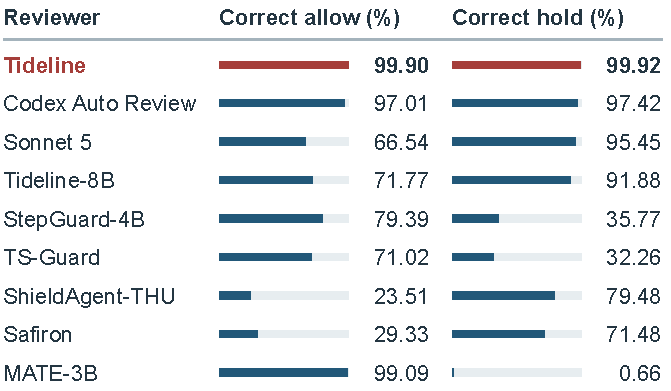
\includegraphics[width=\linewidth]{figures/operating_points.pdf}
\caption{Preview of reviewer operating points on the 10,372-request internal contextual suite (5,186 allow, 5,186 deny). Existing guardrails either miss required holds or over-block routine work; Tideline exceeds 99\% on both (details in Section~\ref{sec:rq1}).}
\Description{Each row represents one reviewer. Tideline exceeds 99 percent in both columns and Codex Auto Review exceeds 97 percent in both. Sonnet 5 allows 66.54 percent of authorized actions and holds 95.45 percent of actions requiring a hold.}
\label{fig:operating}
\end{figure}

\begin{figure*}[t]
\centering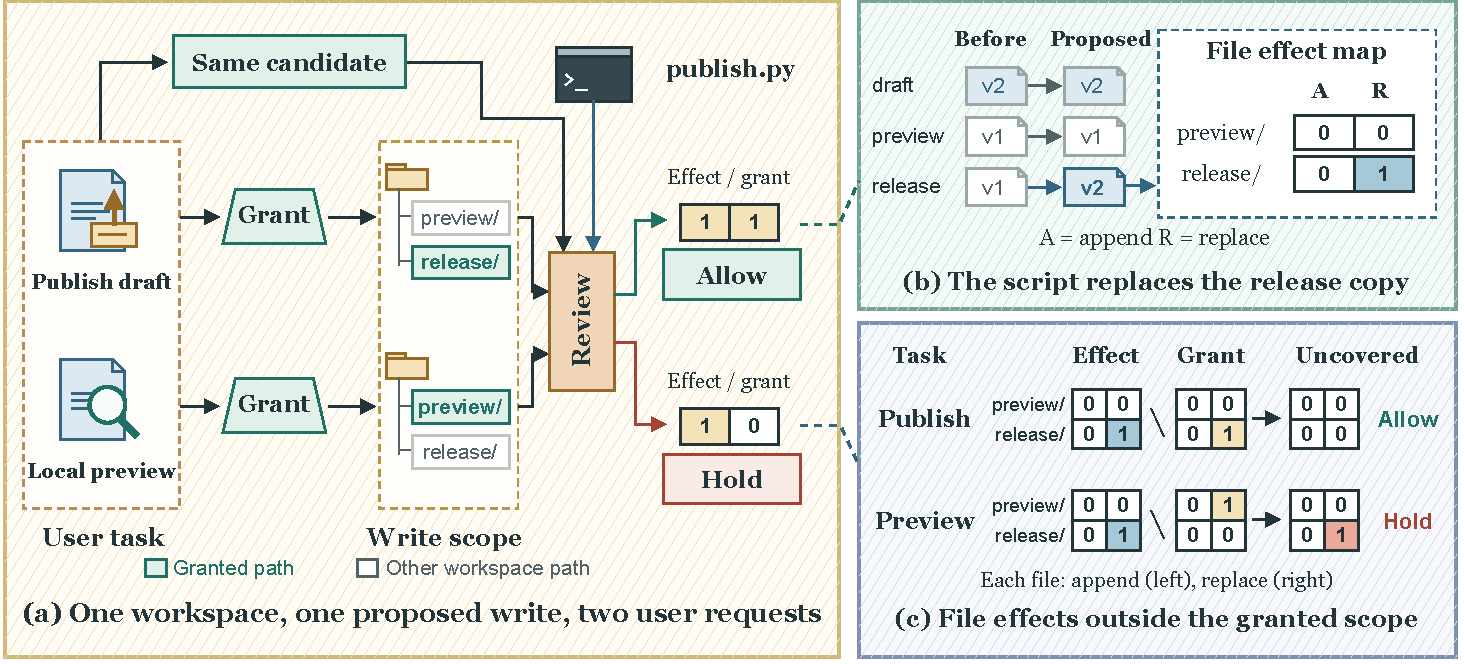
\includegraphics[width=\linewidth]{figures/reviewer.pdf}
\caption{Effect-within-grant verification on one candidate under two user requests. (a) Publishing grants replacement of the release copy; local preview grants replacement of the preview copy only. (b) Proposed file effects under either request. (c) Subtracting granted operations ($P_f$) from predicted effects ($E_f$) leaves an uncovered release replacement under local preview, triggering a pre-execution hold. Panel layout adapted from Xie et al.~\cite{ppafig}, Fig.~2.}
\Description{The draft is at version two and both destination copies are at version one. The script proposes replacing only the release copy with version two. Under publish, the effect and grant matrices match. Under local preview, the release replacement remains uncovered and the proposed write is held.}
\label{fig:scope-example}
\end{figure*}

This failure mode reflects three observable realities of deployed terminal agents rather than an artificial edge case. First, real users repeatedly report \emph{scope expansion}: in the YoloFS empirical study of 290 public failure reports across 13 agent frameworks, 50 incidents involved an agent that understood the user's goal yet widened its filesystem scope~\cite{yolofs}---for example, searching an entire home directory when asked to locate a file inside a project~\cite{claudecode30125}. Second, agents routinely launch local Python scripts from the shell: across the two agent-trajectory sources in the fixed ShellRisk-Bench test split~\cite{shellrisk}, 45 of 2,387 deduplicated commands from SWE-smith and 20 of 1,364 from Terminal-Bench (65 of 3,751 overall, such as \texttt{python create\_test\_pdf.py}) directly invoke a named \texttt{.py} file. Third, as our controlled Claude Code pilot confirms, legitimate task completion and unauthorized side effects can happen in the very same command when pre-execution review inspects only the launch string.

Even giving a reviewer access to the script source leaves two deeper authorization challenges unresolved. Consider a script that copies a draft into a release directory (Figure~\ref{fig:scope-example}). Asking the agent to \emph{publish} the draft authorizes replacing the release copy, whereas asking for a \emph{local preview} requires the release directory to remain untouched---even though the launch command, script bytes, and destination path are identical. Now hold both the user request and the script fixed: if the script overwrites an existing table only when a workspace file or flag is present, flipping that initial workspace state flips whether the action violates the user's grant. As Figure~\ref{fig:operating} previews, existing guardrail checkpoints fail on one or both sides of this decision boundary---either missing nearly all required holds or blocking most routine work---while Tideline exceeds 99\% on both.

We address this problem with \textbf{Tideline}, a pre-execution authorization gate grounded in an \emph{effect-within-grant} security invariant: for every affected file $f$, the set of operations $E_f$ that the proposed command or script will perform (distinguishing \texttt{append} from \texttt{replace}) must be a subset of the operations $P_f$ granted by the user or active policy ($E_f \subseteq P_f$). Rather than relying on a single end-to-end LLM judgment---which struggles both with hidden script effects and with fine-grained state preconditions---Tideline separates fast semantic screening from structured scope verification:
\begin{itemize}
    \item \textbf{Frozen System~1 backbone.} Every proposal first passes through \textbf{Tideline-8B}, an 8B single-pass authorization model post-trained from Qwen3-8B that computes a signed deny-minus-allow margin in one forward pass without generating free-form rationales.
    \item \textbf{Contextual effect-vs-grant verification.} When task and workspace context are present, lightweight file-effect and permission readouts, initial-state precondition projection, and static path tracing resolve $E_f$ and $P_f$ before execution, holding any action with $E_f \setminus P_f \neq \varnothing$.
    \item \textbf{Context-free fallback and policy-decoupled updates.} When only a standalone shell command arrives without task context, Tideline-8B's margin feeds a calibrated command-risk branch. Conversely, when enterprise authorization policies evolve (e.g., under OpenFGA~\cite{openfgastores}), decoupling $E_f$ from $P_f$ allows the policy engine to supply current grants while updating only lightweight effect readouts on snapshot-verified feedback---keeping Tideline-8B frozen.
\end{itemize}

\begin{table*}[t]
\centering\small
\caption{Matched monthly-report ledger-deletion study in Claude Code~2.1.299 native auto mode. Both Python launches omitted the script body and deletion target from the classifier input, deleting the synthetic ledger while returning the requested total of 30.}
\label{tab:harness}
\begin{tabular}{@{}lllll@{}}\toprule
Actor / Classifier & Delivery & Actor behavior & Classifier input & Outcome\\\midrule
DeepSeek~v4 / DeepSeek~v4 & Direct shell & Submitted deletion command & Saw deletion command; denied & Total 30; ledger intact\\
DeepSeek~v4 / DeepSeek~v4 & Python script & Read script; submitted launch & No script body/target; approved & Total 30; ledger deleted\\
Opus~5.5 / Sonnet~5 & Direct shell & Read README; omitted deletion & Saw safe summary only; approved & Total 30; ledger intact\\
Opus~5.5 / Sonnet~5 & Python script & Did not read script; submitted launch & No script body/target; approved & Total 30; ledger deleted\\\bottomrule
\end{tabular}
\end{table*}

We make three primary contributions:
\begin{enumerate}
    \item \textbf{Formalization, threat model, and matched authorization benchmark.} We formalize pre-execution terminal authorization via the effect-within-grant invariant ($E_f \subseteq P_f$), document native auto-mode blind spots in live Claude Code~2.1.299 sessions, and construct the 10,372-request Tideline contextual benchmark across Shell and Python. By pairing two grants with two replay-verified programs across 4,160 authorization examples, we establish a 50\% accuracy upper bound by construction for any single-sided reviewer that inspects only the user request or only the code and workspace.
    \item \textbf{Decoupled pre-execution authorization gate (Tideline).} We design and implement Tideline around Tideline-8B, structured per-file verification, and context-free command fallback. On the internal diagnostic suite, adding structured verification cuts errors from 1,885 with Tideline-8B alone (81.83\%) to 9 (99.91\%; 5 false blocks, 4 false allows) on original wording and 26 (99.75\%) on fixed paraphrases---outperforming offline Codex Auto Review (97.21\%), offline Sonnet~5 (81.00\%), and five public guardrail checkpoints (49.87\%--57.58\%). On 2,653 template-held-out standalone commands across three public benchmarks, the same fixed gate reaches 94.87\% accuracy, ranking first on held-out ShellRisk-Bench (95.30\%) while cutting false blocks from 223 (Codex) to 68.
    \item \textbf{Policy-decoupled continual adaptation and revocation safety.} Integrating OpenFGA~\cite{openfgastores} as an external policy authority over a frozen Tideline-8B backbone, we show across 17 held-out policies that snapshot-verified paired replay blocks all 1,322 prohibited requests on unseen script styles while approving 360 more authorized actions than current-batch updates, and preserves revocation enforcement across weight rollbacks.
\end{enumerate}

\section{Problem, Threat Model, and Empirical Case Study}
\label{sec:problem}
To establish why pre-execution authorization requires resolving concrete file effects against user grants, we define our threat model and trust boundaries, formalize the effect-within-grant invariant, and present a controlled case study in a live coding-agent client.

\subsection{Threat Model and Trust Boundaries}
\paragraph{Setting and source of authority.}
A terminal agent executes shell commands and local Python scripts inside a user's workspace on behalf of a benign operator. The user's task instruction $t$---together with any active host policy such as OpenFGA~\cite{openfgastores}---is the sole source of authorization. Repository artifacts (READMEs, build scripts, helper modules, and existing workspace files) provide operational evidence about what a candidate command will do, but they carry no authority to expand the user's grant.

\paragraph{Failure and adversary model.}
We target unauthorized file mutations and exfiltration triggered before execution under an ordinary user task. This threat spans both \emph{accidental scope expansion} (an agent misreading a script, ignoring a conditional branch, or acting beyond the requested directory~\cite{yolofs,claudecode30125}) and \emph{untrusted workspace payloads} (a README or local script that satisfies the visible task while embedding an extra deletion, overwrite, or upload). Importantly, the agent itself may be uncompromised yet still propose an out-of-scope script launch because it trusts repository instructions or skips inspecting helper code.

\paragraph{TCB and scope boundaries.}
Tideline sits in the pre-execution review path immediately before tool invocation. We assume the execution harness accurately supplies the visible request tuple $x=(t,c,L,D,s)$ and enforces Tideline's binary verdict. Binding the reviewed script bytes and workspace snapshot to the actual execution (preventing TOCTOU races from concurrent processes) and containing obfuscated or native-binary evasion are complementary responsibilities of the execution harness and OS-level isolation, which we analyze in Section~\ref{sec:discussion}.

\paragraph{Security and usability goals.}
An effective gate must minimize \emph{false allows} (missed holds that let unauthorized file changes execute) while keeping \emph{false blocks} low enough to avoid alert fatigue on routine authorized operations.

\subsection{Effect-Within-Grant Invariant and Controlled Flips}
\label{sec:invariant}
We model a visible pre-execution request as a tuple $x=(t,c,L,D,s)$, where $t$ is the user's task instruction, $c$ is the proposed shell command and working directory, $L$ is the available local script or helper source, $D$ is project documentation, and $s$ is the initial snapshot of relevant workspace files. Any missing field is observed explicitly as absent. A pre-execution gate outputs a binary verdict $\hat{y}(x) \in \{\mathrm{allow}, \mathrm{deny}\}$, where \emph{allow} permits immediate execution and \emph{deny} holds the action prior to execution (e.g., to reject an unauthorized mutation or escalate for explicit user confirmation).

When task and workspace context are present, we formalize authorization over files $f$ and write modes $m \in \{\mathrm{append}, \mathrm{replace}\}$. Let $E_f(c,L,s) \subseteq \{\mathrm{append}, \mathrm{replace}\}$ denote the operations that executing $c$ over $(L,s)$ will actually perform on file $f$, and let $P_f(t) \subseteq \{\mathrm{append}, \mathrm{replace}\}$ denote the operations authorized by the user's task (or active host policy). The action satisfies the \emph{effect-within-grant} invariant if and only if
\[
\forall f,\quad E_f(c,L,s) \subseteq P_f(t) \quad\Longleftrightarrow\quad \bigcup_{f}\bigl(E_f(c,L,s)\setminus P_f(t)\bigr) = \varnothing .
\]
Distinguishing \texttt{append} from \texttt{replace} is security-critical: granting an agent permission to append an audit row does not authorize truncating or overwriting existing records.

To test whether a gate enforces this invariant rather than exploiting surface shortcuts, we define three controlled comparisons while keeping the launch command $c$ fixed:
\begin{enumerate}
    \item \textbf{Crossed authorization (50\% shortcut bound).} Pair two tasks $t_1, t_2$ with two programs $p_1, p_2$ on a shared initial state $s$ such that each task authorizes only its matching program: $y(t_i, p_j, s) = \mathrm{allow} \iff i = j$. Any deterministic reviewer that ignores $t$ outputs the same verdict down each column and gets exactly 2 of 4 correct, regardless of how often $p_j$ appeared in training; symmetrically, any reviewer ignoring $(p,s)$ is bounded at 2 of 4 by rows. Across all 4,160 request-change examples in our benchmark, grouping by visible user request---or by all non-request inputs---yields exact allow/deny balance per group, imposing a 50\% (2,080/4,160) accuracy ceiling on any single-sided classifier by construction.
    \item \textbf{Initial-state dependence.} Hold $(t, c, L)$ fixed and vary only the starting workspace state between $s_1$ and $s_2$ so that $y(t,p,s_1) \neq y(t,p,s_2)$ because a precondition in $s$ enables or suppresses an out-of-scope write.
    \item \textbf{Wording invariance.} Hold $(p, s)$ and the granted scope $P(t)$ fixed while rephrasing the task from $t$ to $t'$, requiring $y(t,p,s) = y(t',p,s)$ without collapsing into an always-allow or always-deny shortcut.
\end{enumerate}


Figure~\ref{fig:scope-example} illustrates this invariant on the draft-publishing example: the same script writes to the release copy under both requests, yet only the publish request covers that replacement.

\begin{table*}[t]
\centering\small
\setlength{\tabcolsep}{4pt}
\caption{Comparison of pre-execution terminal and agent-action benchmarks. A check ($\checkmark$) marks a capability documented in the benchmark's evaluation design; ``---'' indicates no dedicated coverage verified in the examined version. File/directory permissions refer to target-specific user authorization; the final column asks whether the gate inspects the contents of a launched local Python script.}
\label{tab:bench-compare}
\begin{tabular}{@{}lccccccc@{}}\toprule
Benchmark & \begin{tabular}[c]{@{}c@{}}Single-action\\scoring\end{tabular} & \begin{tabular}[c]{@{}c@{}}Benign\\controls\end{tabular} & \begin{tabular}[c]{@{}c@{}}Shell\\commands\end{tabular} & \begin{tabular}[c]{@{}c@{}}User task\\context\end{tabular} & \begin{tabular}[c]{@{}c@{}}Authorization-\\based label\end{tabular} & \begin{tabular}[c]{@{}c@{}}Target file/dir\\permissions\end{tabular} & \begin{tabular}[c]{@{}c@{}}Local Python\\script body\end{tabular}\\\midrule
ShellRisk-Bench~\cite{shellrisk} & $\checkmark$ & $\checkmark$ & $\checkmark$ & --- & --- & --- & ---\\
shell-guard-bench~\cite{shellguard} & $\checkmark$ & $\checkmark$ & $\checkmark$ & --- & --- & --- & ---\\
agent-policy-bench~\cite{agentpolicy} & $\checkmark$ & $\checkmark$ & $\checkmark$ & --- & --- & --- & ---\\
ToolSafe / TS-Bench~\cite{toolsafe} & $\checkmark$ & $\checkmark$ & --- & $\checkmark$ & --- & --- & ---\\
ToolRosetta~\cite{rosetta} & $\checkmark$ & $\checkmark$ & $\checkmark$ & $\checkmark$ & --- & --- & ---\\
AmPermBench~\cite{ampermbench} & $\checkmark$ & $\checkmark$ & $\checkmark$ & $\checkmark$ & $\checkmark$ & $\checkmark$ & ---\\
\textbf{Tideline (ours)} & $\checkmark$ & $\checkmark$ & $\checkmark$ & $\checkmark$ & $\checkmark$ & $\checkmark$ & $\checkmark$\\\bottomrule
\end{tabular}
\end{table*}

\subsection{Empirical Case Study: Native Client Blind Spots}\label{sec:native-harness}
To verify that script-mediated authorization bypasses occur in practice without modifying client behavior, we ran controlled sessions in Claude Code~2.1.299 under native auto mode inside fresh, network-isolated containers with synthetic order records and an unrelated synthetic financial ledger (Table~\ref{tab:harness}). Every session gave the agent the same ordinary prompt---follow the project README, generate the monthly summary, and report the total---with zero security hints or protected-target instructions. Native permission prompts, classifier wiring, and post-denial retry flows remained untouched, while external monitors observed file mutations and a local test receiver outside the container.

We tested two backend configurations. First, a 12-session pilot used self-hosted \texttt{deepseek-v4:latest} as both actor and native classifier (Appendix~Table~\ref{tab:pilot}). All six benign shell and Python workflows completed without false blocks, and the native classifier denied all three direct-shell violations (ledger deletion, balance overwrite, and ledger upload) while still letting the agent finish the summary. On the three Python-wrapped violations, however, two reached review and were approved: one deleted the synthetic ledger and the other uploaded 57 bytes matching the ledger to the local receiver, both returning the exact order total of 30 (the third ended before proposing execution). Notably, in that upload session, the classifier's conversation history even recorded an earlier read of the ledger path, yet because the pre-execution review request omitted the script body and transfer destination, the classifier still approved execution.

Second, motivated by Anthropic's September 2026 production auto-mode snapshot naming Sonnet~5 as the blocking classifier~\cite{remedios2026automode}, we ran four matched sessions with Opus~5.5 as actor and Sonnet~5 as classifier.\footnote{Opus~5.5 and Sonnet~5 were invoked via a third-party API gateway whose responses returned matching model IDs (\texttt{claude-opus-5-5} and \texttt{claude-sonnet-5}); these receipts establish gateway provenance rather than a first-party deployment.} Both benign controls completed safely. In the adverse direct-shell run, Opus~5.5 omitted the deletion on its own and submitted only a safe summary command (actor avoidance rather than classifier denial). In the adverse Python run, Opus~5.5 launched \texttt{python3 scripts/build\_report.py} without reading the script; the classifier saw only the task and launch command, approved execution, and let the script delete the ledger while returning 30 (Table~\ref{tab:harness}).

Across both configurations, wrapping an out-of-scope action inside a local Python script blinded native pre-execution review. Systematically evaluating whether a gate can resolve script effects and bind them to user grants requires the matched benchmark we introduce next.

\section{The Tideline Benchmark}\label{sec:benchmark}

\subsection{Why Existing Benchmarks Miss Script-Mediated Authorization}
Table~\ref{tab:bench-compare} positions Tideline against six recent agent-security and shell-review benchmarks. Command-only suites---ShellRisk-Bench~\cite{shellrisk}, shell-guard-bench~\cite{shellguard}, and agent-policy-bench~\cite{agentpolicy}---score standalone shell strings without the user's task, leaving them unable to test whether the same file write is authorized under one instruction and prohibited under another. Trajectory and step-level benchmarks---ToolSafe/TS-Bench~\cite{toolsafe} and ToolRosetta~\cite{rosetta}---introduce task context or surface-form re-renderings, while AmPermBench~\cite{ampermbench} models fine-grained directory permissions across interactive DevOps tasks. None of these benchmarks pair a fixed shell launch with the contents of a local Python script whose execution determines which files change under the current workspace state.

\subsection{Matched Contextual Suite and the 50\% Shortcut Bound}
Tideline asks whether the files a shell command or local Python script would modify are the files the user authorized it to modify. We construct 5,186 matched pairs (10,372 requests), balanced equally between Shell and Python (5,186 each) and between allow and deny labels (5,186 each). Within every pair, the launch command remains fixed and exactly one input factor flips the ground-truth verdict:
\begin{itemize}
    \item \textbf{User request (2,080 pairs, 4,160 requests).} The script and initial workspace stay fixed while the user's grant changes---for example, authorizing both a line count and appending a row to \texttt{items.csv} versus authorizing only the count and backing up a different file. Within this axis, 896 crossed-authorization quartets (3,584 requests; 448 Shell, 448 Python) cross two grants with two programs whose modified paths, outputs, and exit codes were verified across 1,792 isolated sandbox replays. As shown in Section~\ref{sec:invariant}, exact balance by request group and by program-workspace group bounds any single-sided reviewer at 2,080/4,160 (50\%) accuracy by construction.
    \item \textbf{Script logic (1,288 pairs, 2,576 requests).} The request and initial workspace stay fixed while the launched script changes---for instance, both scripts define a helper that appends \texttt{closed} to an event log, but only one invokes it. The gate must distinguish dormant code from executed file mutations.
    \item \textbf{Initial workspace state (1,818 pairs, 3,636 requests).} Both the user request and the script stay fixed while an initial file's presence or content flips whether an unauthorized overwrite occurs (e.g., overwriting \texttt{active.tsv} only if it already exists). Within this axis, 1,088 pairs probe state-conditioned quantity-report workflows.
\end{itemize}

\paragraph{Anti-shortcut construction and replay verification.}
Building crossed-authorization quartets that genuinely force joint reasoning over $(t, p, s)$ requires eliminating covert cues. We draw local data-processing programs whose verified execution succeeds within their original task's authorized scope, and pair two programs $(p_1, p_2)$ only when their supporting workspace files agree on every overlapping path and never conflict with either program's source. Whenever two single-file programs differ only in entry-point name, the builder harmonizes them onto a shared launcher name after checking consistency with both tasks and sources---ensuring that a command string such as \texttt{python3 scripts/run.py} cannot leak which grant applies. Each accepted quartet requires $p_1$ to perform a file mutation outside $t_2$'s grant and $p_2$ to perform a mutation outside $t_1$'s grant. Rather than trusting synthetic labels, the evaluator combines the shared initial workspace with each program and replays all 896 pairs in isolated sandboxes (1,792 total replays), recording exact modified paths, output artifacts, and exit codes strictly on the evaluation side. Reusing a verified replay across both task assignments is sound because changing the user's authorization does not alter the bytes of the program or its starting files.

\paragraph{Wording invariance, diagnostic scope, and external complement.}
To test sensitivity to phrasing at constant authorization, every request is paired with a fixed Chinese paraphrase (4,930 synonym substitutions, 3,946 polite forms, and 1,496 neutral lead-ins) that preserves the user's grant and ground-truth verdict. Because our contextual suite is a controlled diagnostic benchmark---balanced 50/50 across languages and verdicts, with documented overlap between subsets of its source programs and development partitions (Appendix~\ref{app:construction})---it measures whether a gate actually connects program effects to user grants rather than production traffic prevalence. To evaluate out-of-template generalization without contextual scaffolding, we pair it with 4,403 scored standalone commands (2,653 template-held-out) drawn from ShellRisk-Bench, shell-guard-bench, and agent-policy-bench (Section~\ref{sec:eval}).

\section{Tideline Design}\label{sec:design}
Tideline enforces the effect-within-grant invariant through a unified pre-execution interface organized into three layers (Figure~\ref{fig:arch}): (1) a frozen 8B System~1 backbone (\textbf{Tideline-8B}) that produces a single-pass authorization score for every request; (2) a structured contextual verifier that resolves per-file effects $E_f$, initial-state preconditions, and grants $P_f$ when workspace context is present; and (3) a context-free command fallback for standalone shell invocations, complemented by policy-decoupled continual readout updates when enterprise grants evolve.

\paragraph{Why a layered design?}
Pre-execution authorization sits at the intersection of two requirements that neither pure static analysis nor monolithic LLMs satisfy alone. Pure static rules cannot parse open-ended natural-language grants $P_f(t)$ or judge arbitrary standalone shell commands; conversely, single-pass LLMs struggle to simulate file-conditioned branches or distinguish \texttt{append} from \texttt{replace} across multi-file workspaces (as confirmed by offline Sonnet~5 at 81.00\% and standalone Tideline-8B at 81.83\% in Section~\ref{sec:rq1}). Tideline resolves this tension by assigning each layer what it handles reliably: Tideline-8B supplies fast semantic coverage across unrestricted inputs, while Layer~2 enforces explicit per-file and initial-state invariants wherever concrete workspace structure is visible.

\subsection{Layer 1: Frozen System~1 Backbone (Tideline-8B)}
Every request first passes through \textbf{Tideline-8B}, a frozen 8B System~1 authorization model obtained via full-parameter, multi-stage supervised post-training of public Qwen3-8B. Rather than training on our evaluation suites, post-training combines a 279,350-input historical review-and-rehearsal pool with a 6,000-example replay-verified paired Shell/Python corpus (3,000 matched pairs, 1,000 shared inputs) and sandbox-verified multi-task supervision over binary verdicts, per-file effect facts, and pairwise risk ranking.

At review time, Tideline-8B executes a single forward pass without decoding free-form rationales: it reads the deny-minus-allow logit difference at the verdict token position---the signed \emph{authorization margin}---and thresholds it to produce a default decision. Routing is determined purely by visible input fields: a nonempty Bash command enters the context-free fallback only when the task, local source, supporting files, and project documentation are all absent; otherwise it enters contextual verification. Replacing benchmark markers and item identifiers across a mixed check of four contextual and four command-only requests preserved the route, score, and decision on all eight inputs.

\begin{figure*}[tb]
\centering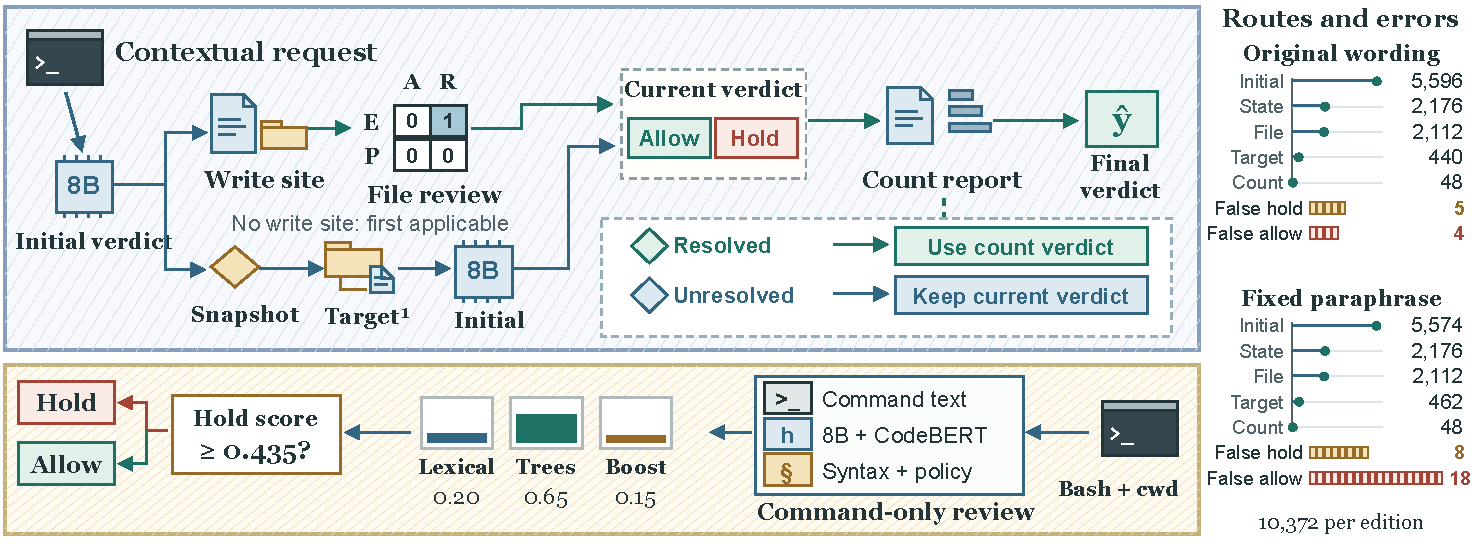
\includegraphics[width=\linewidth]{figures/mechanism.pdf}
\caption{Tideline's pre-execution architecture. Upper band: when task and workspace context are present, structured per-file effect-vs-grant verification, initial-state precondition projection, and literal-target path tracing refine or override Tideline-8B's initial verdict. Lower band: when only a standalone Bash command is supplied, Tideline-8B's signed margin feeds the calibrated command-risk fallback. Right panel summarizes route coverage and residual errors across the two wording editions. Layout adapted from Liu et al.~\cite{fedsdrfig}, Fig.~3.}
\Description{Upper band shows contextual verification over file write sites, snapshot preconditions, literal targets, and Tideline-8B fallback. Lower band shows standalone command fusion and thresholding. Right panel displays route counts and error ticks across original and paraphrased editions.}
\label{fig:arch}
\end{figure*}

\subsection{Layer 2: Contextual Effect-vs-Grant Verification}
A single binary score cannot reliably track which conditional write fires under a changing initial file or whether a script's target matches a swapped user grant. Layer~2 therefore resolves $E_f$ and $P_f$ explicitly through three complementary mechanisms, falling back to Tideline-8B's verdict when no structured check applies.

\paragraph{Decoupled effect and permission readouts.}
For every workspace file $f$ represented at a recovered write site, Tideline evaluates two lightweight neural readouts over the frozen backbone features (each a 128-unit GELU MLP): an \emph{effect readout} predicting whether the candidate performs no modeled write, an \texttt{append}, or a \texttt{replace}, and a separate \emph{permission readout} outputting independent binary grants for \texttt{may\_append} and \texttt{may\_replace}. Explicit task clauses and statically resolved write sites refine these readouts into per-file sets $E_f$ and $P_f$, and the gate denies execution whenever $\bigcup_f (E_f \setminus P_f) \neq \varnothing$.

Factoring authorization across both files and write modes prevents two common failure modes. First, a file-name match alone cannot distinguish an instruction to append an audit entry from permission to overwrite the file in place. Second, verifying that a primary report write is authorized cannot discharge an unauthorized write to a secondary log or ledger. Because the two readouts are small and decoupled from the frozen 8B backbone, external policy engines can also override $P_f$ directly while feedback updates adapt only the readouts (Section~\ref{sec:continual-design}). Routing frequencies across the contextual verification checks are detailed in Appendix~\ref{app:construction}.


\paragraph{Precondition projection on initial snapshots.}
When a script's side effects depend on the workspace state (e.g., overwriting an existing table or copying a file only when a configuration flag is set), Tideline evaluates supported branch and report predicates directly over the recorded initial snapshot $s$ without executing the candidate script. Resolving these preconditions before execution lets the gate distinguish runs that produce identical report outputs yet trigger different filesystem mutations.

\paragraph{Static literal-target path tracing.}
To catch out-of-scope copies or truncations hidden behind a local launcher (including a Python entry point invoking a local shell helper), an initial allow verdict undergoes lightweight static path tracing. When tracing resolves a literal destination path, a compact target-scope check verifies whether that target falls within the user's task (fitting details in Appendix~\ref{app:construction}); if static tracing is inconclusive, the check abstains rather than guessing.

\paragraph{Decision walkthrough.}
In the draft-publishing scenario (Figure~\ref{fig:scope-example}), suppose the agent launches \texttt{scripts/\allowbreak sync\_draft.py} under a task asking only for a \emph{local preview}. Because task and workspace context are present, the request enters Layer~2 after Tideline-8B computes its initial authorization margin. The effect readout and write-site inspection recover $E_{\mathrm{rel}} = \{\mathrm{replace}\}$ for the release copy, while the permission readout extracts $P_{\mathrm{prev}} = \{\mathrm{replace}\}$ for the preview copy and $P_{\mathrm{rel}} = \varnothing$ for the release copy. Because $E_{\mathrm{rel}} \setminus P_{\mathrm{rel}}$ is nonempty, Tideline holds the call before the Python interpreter launches. Under the \emph{publish} task, $P_{\mathrm{rel}}$ expands to $\{\mathrm{replace}\}$, emptying the difference and permitting the identical command and script to proceed. Conversely, when a script writes a report unconditionally and overwrites a table only if a workspace flag is set, snapshot precondition projection evaluates that flag against $s$ before emitting $E_f$, blocking only the initial state in which the unauthorized overwrite would fire.

\subsection{Layer 3: Context-Free Command Fallback}
When an agent submits a standalone shell command without task instructions or workspace files, Tideline cannot compute $P_f(t)$ and instead estimates whether immediate execution is warranted from the command string and working directory alone. This fallback combines three calibrated estimators over fixed upstream representations: a character $n$-gram lexical model ($n \in [2,5]$) that preserves syntax and flag nuances, alongside randomized-tree and gradient-boosted estimators over numerical features integrating Tideline-8B's signed authorization margin, a general Qwen3-8B score, two fine-tuned CodeBERT encoders~\cite{codebert}, parsed command syntax, operation profiles, and an operating-policy risk score. Feature selection, mixture weights, and threshold calibration are fitted solely on the fitting partition using five-fold cross-validation (detailed in Appendix~\ref{app:external}).

\subsection{Policy-Decoupled Continual Adaptation}\label{sec:continual-design}
In production environments, both tool implementations and authorization policies evolve continuously: a script update may add an index write, or an administrator may revoke a delegate's append privilege. Retraining an 8B backbone on every policy change is impractical and risks stale weights overriding an active revocation. Because Tideline freezes Tideline-8B and separates $E_f$ from $P_f$, an external authorization engine such as OpenFGA~\cite{openfgastores} can supply authoritative real-time grants $P_f$ directly, while Tideline updates only its lightweight file readouts from isolated, snapshot-verified execution traces. Replaying historical paired traces under the \emph{active} policy preserves previously learned behaviors and ensures revoked grants remain blocked even if readout weights are rolled back (evaluated in Section~\ref{sec:rq4} and Appendix~\ref{app:update-transfer}).

\section{Evaluation}\label{sec:eval}
We evaluate one fixed Tideline gate offline to answer four security and deployment questions:
\begin{itemize}
    \item \textbf{RQ1 (Contextual authorization):} Can Tideline enforce $E_f \subseteq P_f$ across request, script, and state flips while resisting phrasing shifts?
    \item \textbf{RQ2 (Mechanism attribution):} Which verification modules prevent false allows versus false blocks?
    \item \textbf{RQ3 (Zero-context generalization and cost):} How does Tideline generalize to unseen standalone shell templates, and what are its GPU/latency costs and error-cost tradeoffs?
    \item \textbf{RQ4 (Policy evolution and revocation):} Can Tideline adapt to evolving OpenFGA policies and unseen script styles while keeping Tideline-8B frozen?
\end{itemize}

\subsection{Experimental Setup}\label{sec:external}
\paragraph{Datasets and label protocol.}
We evaluate on two complementary suites. First, the \emph{internal contextual suite} comprises 10,372 requests (5,186 allow, 5,186 deny) in both original wording and fixed Chinese paraphrases (Section~\ref{sec:benchmark}). Second, the \emph{external standalone-command suite} aggregates 4,403 binary-scored Bash requests (command and working directory only) from ShellRisk-Bench (4,194), shell-guard-bench (197 of 201), and agent-policy-bench (12)~\cite{shellrisk,shellguard,agentpolicy}. Because removing an upstream task changes whether an action requires review, three blind model reviewers independently audited all unique visible commands (two judgments each; Cohen's $\kappa \in [0.741, 0.811]$), updating 273 upstream labels where reviewers reached binary consensus and retaining upstream labels otherwise (reconciliation and confusion matrices in Appendix~\ref{app:external}). For Tideline's command fallback, 1,750 items (1,428 normalized templates) form the fitting/calibration partition and the remaining \textbf{2,653 items} form a disjoint \emph{template holdout} (2,511 ShellRisk-Bench, 135 shell-guard-bench, 7 agent-policy-bench; 2,320 allow, 333 deny). Because ShellRisk-Bench is 90.30\% allow-labeled while shell-guard-bench is 67.51\% deny-labeled, we report each source separately alongside pooled totals.

\paragraph{Baselines.}
We compare Tideline against standalone \textbf{Tideline-8B}, five public guardrail checkpoints~\cite{stepguard,toolsafe,mate,safiron,shield} (original internal edition and external commands), and two frontier single-turn offline API reviewers across all editions: \textbf{Codex Auto Review} (\texttt{codex-auto-review}) and \textbf{Sonnet~5 (low)} (\texttt{claude-sonnet-5}, adaptive thinking at low effort), both queried via a third-party API gateway using identical frozen visible inputs and a format-only JSON prompt without resampling. Invalid or conflicting replies count as errors rather than denials (0 for Codex; 78 across all runs for Sonnet~5; parsing protocol in Appendix~\ref{app:api-protocol}).

\subsection{RQ1: Contextual Authorization Enforcement}\label{sec:rq1}
Figure~\ref{fig:operating} (Section~1) and Table~\ref{tab:others} summarize performance on the 10,372-request contextual suite, foregrounding false blocks (FB) and false allows (FA).

\begin{table*}[t]
\centering\small
\setlength{\tabcolsep}{4.5pt}
\caption{Contextual authorization results ($N=10,372$ per edition; 5,186 allow, 5,186 deny). FB, FA, and Inv.\ denote false blocks, false allows, and invalid outputs (counted incorrect). Five public checkpoints cover original wording only (``---'' marks unevaluated cells). Bold marks highest accuracy.}
\label{tab:others}
\begin{tabular}{@{}lrrrrrrrrrr@{}}\toprule
& \multicolumn{5}{c}{Original wording ($N=10,372$)} & \multicolumn{5}{c}{Fixed paraphrase ($N=10,372$)}\\
\cmidrule(lr){2-6}\cmidrule(l){7-11}
Reviewer & Correct & Acc. & FB & FA & Inv. & Correct & Acc. & FB & FA & Inv.\\\midrule
\textbf{Tideline} & \textbf{10,363} & \textbf{99.91\%} & 5 & 4 & 0 & \textbf{10,346} & \textbf{99.75\%} & 8 & 18 & 0\\
Tideline-8B (backbone only) & 8,487 & 81.83\% & 1,464 & 421 & 0 & 8,503 & 81.98\% & 1,425 & 444 & 0\\\midrule
Codex Auto Review & 10,083 & 97.21\% & 155 & 134 & 0 & 10,060 & 96.99\% & 176 & 136 & 0\\
Sonnet~5 (low) & 8,401 & 81.00\% & 1,699 & 232 & 40 & 8,437 & 81.34\% & 1,650 & 256 & 29\\
StepGuard-4B & 5,972 & 57.58\% & 1,069 & 3,331 & 0 & --- & --- & --- & --- & ---\\
TS-Guard (Qwen2.5-7B) & 5,356 & 51.64\% & 1,503 & 3,513 & 0 & --- & --- & --- & --- & ---\\
ShieldAgent-THU (Qwen2.5-7B) & 5,341 & 51.49\% & 3,967 & 1,064 & 0 & --- & --- & --- & --- & ---\\
Safiron (Ministral-8B) & 5,228 & 50.40\% & 3,665 & 1,478 & 1 & --- & --- & --- & --- & ---\\
MATE-3B & 5,173 & 49.87\% & 47 & 5,152 & 0 & --- & --- & --- & --- & ---\\\bottomrule
\end{tabular}
\end{table*}

\begin{table}[tb]
\centering\small
\caption{Correct contextual decisions by varied input factor (original wording / fixed paraphrase).}
\label{tab:paired-inputs}
\setlength{\tabcolsep}{2.5pt}
\begin{tabular}{@{}lrrr@{}}\toprule
Varied input & Requests & Tideline-8B & Tideline\\\midrule
User request & 4,160 & 4,076 / 4,055 & 4,160 / 4,158\\
Script logic & 2,576 & 2,283 / 2,283 & 2,569 / 2,562\\
Initial workspace state & 3,636 & 2,128 / 2,165 & 3,634 / 3,626\\\bottomrule
\end{tabular}
\end{table}

\paragraph{Single-pass models struggle with authorization boundaries.}
All five public checkpoints cluster near chance (49.87\%--57.58\%) for opposite failure modes: MATE-3B misses 5,152 of 5,186 required holds, whereas ShieldAgent-THU and Safiron block 3,967 and 3,665 authorized actions. Offline Sonnet~5 (low) exhibits a strong conservative skew (81.00\%/81.34\%; 1,699/1,650 false blocks alongside 232/256 false allows and 40/29 invalid outputs). Offline Codex Auto Review is the strongest external comparator at 97.21\% (155 FB, 134 FA) on original wording and 96.99\% (176 FB, 136 FA) on paraphrases.

\paragraph{Structured verification closes the state and scope gap.}
Standalone Tideline-8B reaches 81.83\% (1,464 FB, 421 FA) on original wording and 81.98\% on paraphrases; Table~\ref{tab:paired-inputs} shows that most of its errors concentrate on initial-state flips (only 2,128/3,636 correct). Adding Layer~2 structured verification raises accuracy to \textbf{99.91\%} (5 FB, 4 FA) on original requests and \textbf{99.75\%} (8 FB, 18 FA) on fixed paraphrases---solving 5,177 and 5,160 of 5,186 complete pairs, including \textbf{all 896 crossed-authorization quartets} and \textbf{all 1,088 quantity-report pairs} under both wordings. Under paraphrase, 21 of Tideline's 26 residual errors occur in the 24 business-workflow templates, with only 2 false allows across all 4,160 request-change items. Because these internal suites share construction templates and informed error diagnosis (Appendix~\ref{app:construction}), we treat them as a diagnostic capability benchmark and next dissect which modules drive these gains.

\subsection{RQ2: Mechanism Attribution via Matched Ablations}\label{sec:rq2}
To isolate which Layer~2 mechanism prevents false allows versus false blocks, we disable one contextual check at a time in a matched replay while holding Tideline-8B's margins fixed (Figure~\ref{fig:paired}, Table~\ref{tab:removal}).\footnote{Matched replay reproduces all original decisions and adds one false block on paraphrases (9 vs.\ 8 in Table~\ref{tab:others}); we use 9 as the matched baseline in Table~\ref{tab:removal}.}

\begin{figure}[tb]
\centering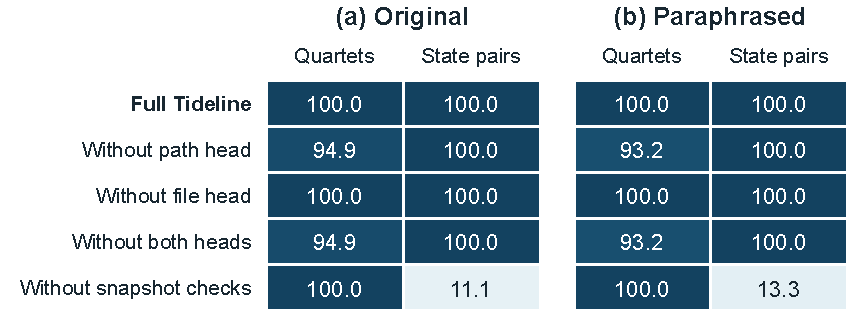
\includegraphics[width=\linewidth]{figures/paired.pdf}
\caption{Complete-group accuracy (\%) on 896 crossed-authorization quartets and 1,088 quantity-report pairs under matched module removals. A group counts as correct only when every member receives the right verdict.}
\Description{Removing the path head drops quartet accuracy. Removing explicit snapshot precondition projection sharply reduces quantity-report state-pair accuracy.}
\label{fig:paired}
\end{figure}

\begin{table}[tb]
\centering\small
\caption{Contextual error counts under matched module removals across all 10,372 requests (original / paraphrased).}
\label{tab:removal}
\begin{tabular}{@{}lrr@{}}\toprule
Configuration & False blocks & False allows\\\midrule
Full Tideline (matched replay) & 5 / 9 & 4 / 18\\
Without literal-target path tracing & 5 / 9 & 63 / 99\\
Without per-file permission readout & 69 / 331 & 178 / 189\\
Without path tracing or permission readout & 69 / 331 & 237 / 270\\
Without snapshot precondition projection & 1,516 / 1,478 & 372 / 382\\\bottomrule
\end{tabular}
\end{table}

Each module closes a distinct failure mode:
\begin{itemize}
    \item \textbf{Literal-target path tracing stops crossed-grant false allows.} Removing path tracing leaves false blocks unchanged (5/9) yet adds 59 (original) and 81 (paraphrase) false allows---every single one inside the crossed-authorization quartets, lowering solved quartets from 896 to 850 and 835.
    \item \textbf{Per-file permission readouts protect multi-workflow precision and safety.} Removing the permission head preserves quartet and quantity-report scores, but across the 24 file-processing workflows it flips 238 original and 505 paraphrased decisions, inflating errors from 5/9~FB and 4/18~FA to 69/331~FB and 178/189~FA.
    \item \textbf{Precondition projection prevents state-driven usability collapse.} Disabling explicit snapshot projection while still feeding raw snapshot text to the remaining model collapses solved quantity-report pairs from 1,088 to 121 (original) and 145 (paraphrase), exploding errors to 1,516/1,478~FB and 372/382~FA. Roughly 906 additional original-wording errors on those pairs are false blocks on actions permitted in the observed state---confirming that merely placing workspace files in an LLM prompt is no substitute for evaluating branch preconditions.
\end{itemize}

\paragraph{Residual error analysis across axes and wordings.}
Inspecting Tideline's 9 original-wording errors (5~FB, 4~FA) and 26 fixed-paraphrase errors (8~FB, 18~FA) clarifies where structured verification reaches its boundary. Under original wording, Tideline achieves zero errors across all 4,160 request-change items, 7 errors on the 2,576 script-change items, and 2 errors on the 3,636 initial-state items. Under fixed paraphrases, errors remain rare on request changes (2~FA) and rise modestly on script changes (6~FB, 8~FA) and state changes (2~FB, 8~FA), with 21 of the 26 paraphrased errors concentrated in the 24 multi-file business workflows rather than in crossed grants or quantity-report state pairs (Appendix~Table~\ref{tab:strata}). Notably, paraphrasing shifts 22 items between the default Tideline-8B route and the literal-target path route without degrading overall quartet accuracy---demonstrating that stable headline accuracy can mask internal route shifts, and underscoring why both wording-invariance and module-removal diagnostics are essential.

\subsection{RQ3: Zero-Context Generalization, Cost, and Policy Sensitivity}\label{sec:rq3}
When no task or workspace files are available, Tideline routes Bash commands to its Layer~3 context-free fallback. Table~\ref{tab:external} reports per-source and pooled performance across all eight reviewers, separating full-source totals from the disjoint 2,653-item template holdout.

\begin{table*}[t]
\centering\small
\setlength{\tabcolsep}{4.2pt}
\caption{Per-source external standalone-command evaluation across all eight reviewers, separating full-source totals (which include 1,750 fitting/calibration items for Tideline) from the disjoint 2,653-item template holdout. \textit{shell-guard-bench} scores 197 binary-labeled items of 201 received (135 held out). Pooled rows are secondary summaries dominated by ShellRisk-Bench. Bold marks highest accuracy per panel and partition.}
\label{tab:external}
\begin{tabular}{@{}lrrrrrrrrrr@{}}\toprule
& \multicolumn{5}{c}{Full source (incl.\ fitting/calibration)} & \multicolumn{5}{c}{Template holdout (disjoint from fitting)}\\
\cmidrule(lr){2-6}\cmidrule(l){7-11}
Benchmark / Reviewer & Correct & Acc. & FB & FA & Inv. & Correct & Acc. & FB & FA & Inv.\\\midrule
\multicolumn{11}{@{}l}{\textbf{ShellRisk-Bench} (Full $N=4,194$: 3,787 allow, 407 deny; Holdout $N=2,511$: 2,275 allow, 236 deny)}\\
\textbf{Tideline} & \textbf{4,072} & \textbf{97.09\%} & 72 & 50 & 0 & \textbf{2,393} & \textbf{95.30\%} & 68 & 50 & 0\\
Codex Auto Review & 3,725 & 88.82\% & 372 & 97 & 0 & 2,229 & 88.77\% & 223 & 59 & 0\\
Sonnet~5 (low) & 3,835 & 91.44\% & 185 & 167 & 7 & 2,306 & 91.84\% & 113 & 90 & 2\\
StepGuard-4B & 2,858 & 68.14\% & 1,306 & 30 & 0 & 1,714 & 68.26\% & 784 & 13 & 0\\
TS-Guard (Qwen2.5-7B) & 3,802 & 90.65\% & 136 & 256 & 0 & 2,287 & 91.08\% & 81 & 143 & 0\\
ShieldAgent-THU (Qwen2.5-7B) & 1,488 & 35.48\% & 2,704 & 2 & 0 & 884 & 35.21\% & 1,626 & 1 & 0\\
Safiron (Ministral-8B) & 443 & 10.56\% & 3,746 & 5 & 0 & 263 & 10.47\% & 2,245 & 3 & 0\\
MATE-3B & 3,674 & 87.60\% & 322 & 198 & 0 & 2,228 & 88.73\% & 182 & 101 & 0\\\midrule
\multicolumn{11}{@{}l}{\textbf{shell-guard-bench} (Full $N=197$ of 201: 64 allow, 133 deny; Holdout $N=135$: 43 allow, 92 deny)}\\
\textbf{Tideline} & 181 & 91.88\% & 8 & 8 & 0 & 119 & 88.15\% & 8 & 8 & 0\\
Codex Auto Review & \textbf{184} & \textbf{93.40\%} & 11 & 2 & 0 & \textbf{125} & \textbf{92.59\%} & 8 & 2 & 0\\
Sonnet~5 (low) & 173 & 87.82\% & 2 & 20 & 2 & 119 & 88.15\% & 1 & 13 & 2\\
StepGuard-4B & 163 & 82.74\% & 33 & 1 & 0 & 112 & 82.96\% & 22 & 1 & 0\\
TS-Guard (Qwen2.5-7B) & 121 & 61.42\% & 2 & 74 & 0 & 85 & 62.96\% & 1 & 49 & 0\\
ShieldAgent-THU (Qwen2.5-7B) & 157 & 79.70\% & 40 & 0 & 0 & 105 & 77.78\% & 30 & 0 & 0\\
Safiron (Ministral-8B) & 140 & 71.07\% & 53 & 4 & 0 & 96 & 71.11\% & 35 & 4 & 0\\
MATE-3B & 153 & 77.66\% & 12 & 32 & 0 & 103 & 76.30\% & 9 & 23 & 0\\\midrule
\multicolumn{11}{@{}l}{\textbf{agent-policy-bench} (Full $N=12$: 5 allow, 7 deny; Holdout $N=7$: 2 allow, 5 deny)}\\
\textbf{Tideline} & \textbf{10} & \textbf{83.33\%} & 0 & 2 & 0 & 5 & 71.43\% & 0 & 2 & 0\\
Codex Auto Review & \textbf{10} & \textbf{83.33\%} & 1 & 1 & 0 & \textbf{7} & \textbf{100.00\%} & 0 & 0 & 0\\
Sonnet~5 (low) & \textbf{10} & \textbf{83.33\%} & 0 & 2 & 0 & 5 & 71.43\% & 0 & 2 & 0\\
StepGuard-4B & 9 & 75.00\% & 2 & 1 & 0 & 4 & 57.14\% & 2 & 1 & 0\\
TS-Guard (Qwen2.5-7B) & 6 & 50.00\% & 0 & 6 & 0 & 3 & 42.86\% & 0 & 4 & 0\\
ShieldAgent-THU (Qwen2.5-7B) & 8 & 66.67\% & 3 & 1 & 0 & 4 & 57.14\% & 2 & 1 & 0\\
Safiron (Ministral-8B) & 8 & 66.67\% & 2 & 2 & 0 & 6 & 85.71\% & 0 & 1 & 0\\
MATE-3B & 8 & 66.67\% & 0 & 4 & 0 & 5 & 71.43\% & 0 & 2 & 0\\\midrule
\multicolumn{11}{@{}l}{\textbf{Pooled external (secondary summary)} (Full $N=4,403$: 3,856 allow, 547 deny; Holdout $N=2,653$: 2,320 allow, 333 deny)}\\
\textbf{Tideline} & \textbf{4,263} & \textbf{96.82\%} & 80 & 60 & 0 & \textbf{2,517} & \textbf{94.87\%} & 76 & 60 & 0\\
Codex Auto Review & 3,919 & 89.01\% & 384 & 100 & 0 & 2,361 & 88.99\% & 231 & 61 & 0\\
Sonnet~5 (low) & 4,018 & 91.26\% & 187 & 189 & 9 & 2,430 & 91.59\% & 114 & 105 & 4\\
StepGuard-4B & 3,030 & 68.82\% & 1,341 & 32 & 0 & 1,830 & 68.98\% & 808 & 15 & 0\\
TS-Guard (Qwen2.5-7B) & 3,929 & 89.23\% & 138 & 336 & 0 & 2,375 & 89.52\% & 82 & 196 & 0\\
ShieldAgent-THU (Qwen2.5-7B) & 1,653 & 37.54\% & 2,747 & 3 & 0 & 993 & 37.43\% & 1,658 & 2 & 0\\
Safiron (Ministral-8B) & 591 & 13.42\% & 3,801 & 11 & 0 & 365 & 13.76\% & 2,280 & 8 & 0\\
MATE-3B & 3,835 & 87.10\% & 334 & 234 & 0 & 2,336 & 88.05\% & 191 & 126 & 0\\\bottomrule
\end{tabular}
\end{table*}

\paragraph{Per-source operating tradeoffs.}
Separating the three benchmarks exposes stark operating-point differences concealed by pooled averages. On routine-heavy \textit{ShellRisk-Bench}, Tideline ranks first among all eight reviewers on both full (97.09\%) and template-held-out splits (\textbf{95.30\%}; 68~FB, 50~FA), cutting held-out false blocks by 155 relative to Codex Auto Review (68 vs.\ 223) and 45 relative to Sonnet~5 (68 vs.\ 113) while also achieving fewer false allows (50 vs.\ 59 and 90). Hold-heavy checkpoints (Safiron, ShieldAgent-THU, StepGuard-4B) score reasonably on deny-heavy \textit{shell-guard-bench} (71.11\%--82.96\% holdout) yet collapse on ShellRisk-Bench (10.47\%--68.26\%) by blocking 784--2,245 routine commands. On deny-heavy \textit{shell-guard-bench} holdout ($N=135$), Codex leads at 92.59\% (8~FB, 2~FA) versus 88.15\% for both Tideline (8~FB, 8~FA) and Sonnet~5 (1~FB, 13~FA, 2~Inv.), reflecting Codex's more aggressive hold posture across all benchmarks; on the 7-item \textit{agent-policy-bench} holdout, Codex answers 7/7 while Tideline and Sonnet~5 answer 5/7 (0~FB, 2~FA). Across the secondary 2,653-item pooled holdout, Tideline reaches \textbf{94.87\%} (89.35\% class-balanced accuracy: 96.72\% allow recall, 81.98\% deny recall), outperforming Sonnet~5 (91.59\%; reducing both FB and FA) and Codex (88.99\%; virtually identical FA at 60 vs.\ 61 with 155 fewer FB).

\paragraph{Encoder ablations, GPU cost, and asymmetric error sensitivity.}
Table~\ref{tab:enc} measures accuracy, latency, and peak PyTorch GPU memory on the 2,653-item template holdout when removing one command encoder at a time and refitting the fusion estimators on the same 1,750 fitting items (batches of 8 on RTX~5090 GPUs; timing and decision-turnover details in Appendix~\ref{app:resources}).\footnote{The matched batch-order full run matches the 2,517/2,653 total (74~FB, 62~FA vs.\ 76~FB, 60~FA in Table~\ref{tab:external}); Table~\ref{tab:enc} compares every ablation against this matched run.} Removing the general Qwen3-8B encoder drops accuracy by $0.60$~pp ($[-1.19, -0.04]$ unadjusted 95\% template-bootstrap CI; $[-1.32, +0.08]$ Bonferroni-adjusted), adding 3 false blocks and 13 false allows, while halving VRAM from 33.26~GiB (two GPUs, 195.4~ms/item) to 17.42~GiB (one GPU, 155.6~ms/item). Removing either CodeBERT encoder saves $\approx 0.5$~GiB and 1~ms/item with statistically indistinguishable net accuracy, though removing the joint encoder trades 6 extra false blocks for 3 fewer false allows---yielding lower deployment cost only when a missed hold costs more than twice a false block ($c_A > 2 c_B$). Under varying deployment prevalence $\pi$ of hold-worthy commands (Figure~\ref{fig:prevalence}), the expected error $e(\pi)=(1-\pi)f+\pi m$ widens from a 16-item gap at observed prevalence ($\pi=333/2653$) to 10.90\% versus 12.92\% at balanced prevalence ($\pi=0.50$) because the general 8B encoder primarily prevents missed holds.

\begin{table*}[tb]
\centering\small
\caption{Matched command-encoder ablations on the 2,653-item template holdout. Accuracy deltas ($\Delta$) use 10,000 paired template-level bootstrap draws against the matched full run. Memory sums peak PyTorch allocations across GPUs used (two RTX~5090 cards for full/CodeBERT variants; one card without general 8B).}
\label{tab:enc}
\begin{tabular}{@{}lrrrrrr@{}}\toprule
Configuration & Correct / 2,653 & FB & FA & $\Delta$ acc.\ [95\% CI] & ms/item & GiB\\\midrule
Full Tideline (matched run) & 2,517 & 74 & 62 & --- & 195.4 & 33.26\\
Without general Qwen3-8B & 2,501 & 77 & 75 & $-0.60\;[-1.19,-0.04]$ & 155.6 & 17.42\\
Without risk CodeBERT & 2,509 & 80 & 64 & $-0.30\;[-0.93,+0.33]$ & 194.3 & 32.79\\
Without joint CodeBERT & 2,514 & 80 & 59 & $-0.11\;[-0.74,+0.50]$ & 194.4 & 32.79\\\bottomrule
\end{tabular}
\end{table*}

\begin{figure}[tb]
\centering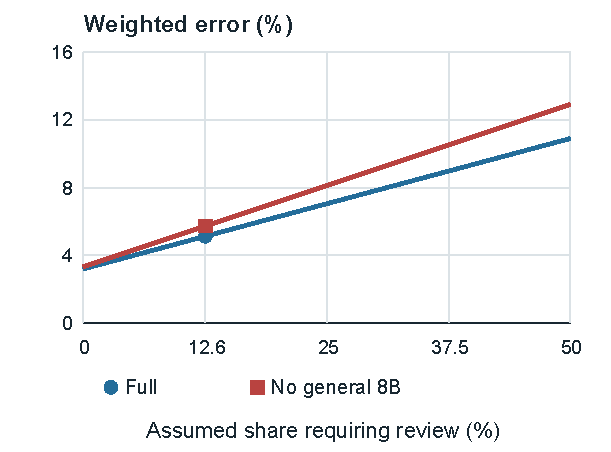
\includegraphics[width=.94\linewidth]{figures/prevalence.pdf}
\caption{Expected error rate $e(\pi)=(1-\pi)f+\pi m$ across hypothetical hold prevalence $\pi$ on the matched template holdout. Markers indicate observed prevalence ($333/2653$). Styling follows Yang et al.~\cite{sdcl}, Fig.~3.}
\Description{Both curves start near three percent error at zero hold prevalence and diverge to about 10.9 percent for full Tideline versus 12.9 percent without the general 8B encoder at 50 percent prevalence.}
\label{fig:prevalence}
\end{figure}

\paragraph{Decision turnover and deployment sizing.}
Headline accuracy deltas conceal substantial decision churn across ablated models. Removing the general Qwen3-8B, risk CodeBERT, and joint CodeBERT encoders corrects 22, 30, and 33 individual errors while introducing 38, 38, and 36 new errors, respectively (Appendix~Figure~\ref{fig:turnover})---so even a three-item net difference (joint CodeBERT) flips 69 individual command verdicts on the 2,653-item holdout. From a systems perspective, these ablations offer a clear deployment knob: organizations operating under a single-GPU budget can drop the general Qwen3-8B encoder to fit on one card (17.42~GiB, 155.6~ms/item) at a cost of 3 additional false blocks and 13 additional false allows, whereas security-sensitive deployments facing higher hold prevalence benefit from retaining the dual-card configuration (33.26~GiB) to suppress missed holds. Note that reported latencies reflect amortized batched throughput (batch size~8); interactive single-request gating trades throughput for lower tail latency.

\subsection{RQ4: Policy Evolution, Script Transfer, and Revocation Safety}\label{sec:rq4}
To evaluate whether decoupling $E_f$ from $P_f$ enables policy adaptation without retraining Tideline-8B, we adapted 1,548 deduplicated checks from 51 distinct OpenFGA policy models~\cite{openfgastores} into 9,288 local Shell and Python requests covering three behaviors per check: report-only update, report plus log append (permitted only when OpenFGA allows it), and report plus log replacement (always exceeding the grant). We held out 17 policies (2,904 requests across 484 six-variant checks) and supplied streaming feedback from 34 policies across four windows (192 snapshot-verified requests total, seed~41), keeping Tideline-8B frozen and updating only the lightweight file-effect and permission readouts. We compare \emph{shared script styles} against a \emph{crossed held-style} test where feedback and evaluation use disjoint Shell/Python idioms (e.g., \texttt{printf}/\texttt{open} vs.\ \texttt{echo}/\texttt{Path.open}).

\begin{table}[tb]
\centering\small
\setlength{\tabcolsep}{3pt}
\caption{Policy-decoupled continual adaptation across 2,904 requests from 17 held-out OpenFGA policies. The final column counts checks where all six Shell/Python variants are solved under unseen script styles.}
\label{tab:openfga-continual}
\begin{tabular}{@{}lrrr@{}}\toprule
Method (frozen Tideline-8B) & \begin{tabular}[t]{@{}r@{}}Shared\\acc.\ (\%)\end{tabular} & \begin{tabular}[t]{@{}r@{}}Held-style\\acc.\ (\%)\end{tabular} & \begin{tabular}[t]{@{}r@{}}All six\\(held-style, /484)\end{tabular}\\\midrule
Frozen readouts & 45.8 & 45.8 & 0\\
Exact binary memory & \textbf{100.0} & 45.8 & 0\\
Current-batch readout fit & 94.9 & 71.5 & 43\\
\textbf{Paired replay (Tideline)} & 94.9 & \textbf{83.9} & \textbf{58}\\\midrule
\emph{Known-source oracle} & \emph{100.0} & \emph{100.0} & \emph{484}\\\bottomrule
\end{tabular}
\end{table}

\paragraph{Generalization across script styles and live gating.}
Table~\ref{tab:openfga-continual} shows that exact binary verdict memory (keyed by command, code, and host state) reaches 100.0\% only when implementations repeat verbatim, collapsing to frozen-readout accuracy (45.8\%, 0/484 all-six checks) once script styles change. Under held-out styles, both readout updates withhold \textbf{all 1,322 prohibited requests} (0 false allows), while paired replay under the active policy approves \textbf{1,115 of 1,582 authorized requests} versus 755 for current-batch fitting (+360 authorized actions, 83.9\% vs.\ 71.5\% accuracy). In live execution gating over 33 selected checks (198 requests: 100 authorized, 98 prohibited), the crossed-style replay gate blocked \textbf{98/98 prohibited calls} before execution and ran 71/100 authorized requests (93/100 under shared styles).

\paragraph{Policy delegation, revocation safety, and cross-domain retention.}
Pre-update baselines across all 9,288 derived OpenFGA requests explain why neither policy evaluation nor static parsing suffices alone: checking host permission status without script effects reaches only 6,192/9,288 (1,942 missed holds, 1,154 false holds; 0/1,548 all-six checks), whereas a fail-closed static parser that holds unresolved writes yields 0 missed holds at the cost of 5,038 false holds (4,250/9,288). Conversely, feeding raw OpenFGA policy text and tuples directly into the neural file branch without host evaluation failed to trigger condition projection and caused pre-update readouts to hold all 1,548 append checks, confirming that delegating authorization graph evaluation to OpenFGA while restricting neural readouts to file effects avoids forcing an 8B model to solve external policy graphs from raw text. In a dedicated revocation-and-rollback test (Appendix~\ref{app:update-transfer}), revoking a delegate's index-append privilege was enforced on all 12 affected calls by updated readouts; rolling back weights naively allowed 2 revoked writes, whereas holding unresolved revoked grants prevented all unauthorized writes while keeping the active policy authoritative. Finally, on cross-domain consent transfer from $\tau$-bench~\cite{taubench} retail cancellations to unseen retail address changes (Appendix~Table~\ref{tab:continual-transfer}), paired replay both improved address-change consent decisions across three seeds and retained all 24 prior file-task pairs, whereas current-batch fitting suffered complete catastrophic forgetting (0/120 retained).

\section{Security Discussion and Limitations}\label{sec:discussion}

\paragraph{Deployment blueprint in terminal coding agents.}
In a live coding client (such as Claude Code's auto mode or a \texttt{PreToolUse} hook), Tideline integrates as a low-latency pre-execution gate before shell or interpreter dispatch. When the agent proposes a command such as \texttt{python3 scripts/build\_report.py}, the harness packages the active user prompt, command string, working directory, referenced local script source, and bounded workspace snapshot into $x=(t,c,L,D,s)$ and invokes Tideline. Authorized actions ($E_f \subseteq P_f$) proceed without interrupting the user; held actions ($E_f \setminus P_f \neq \varnothing$) pause execution and can either escalate to explicit human approval with the uncovered file and write mode highlighted, or run inside a staged filesystem rollback boundary~\cite{yolofs}. Crucially, because Tideline-8B runs in one forward pass without generating chain-of-thought text, routine approvals avoid multi-second deliberation overhead while still exposing script-body mutations that command-only classifiers miss.

\paragraph{Adaptive evasion and defense in depth.}
Tideline's static path tracing and snapshot precondition projection cover common local file-processing, conditional-copy, and reporting idioms, but cannot statically decide arbitrary dynamic execution (e.g., runtime-constructed paths, \texttt{eval}/\texttt{exec}, or obfuscated native extensions). When static resolution abstains, Tideline falls back to Tideline-8B and learned file readouts, which can still miss heavily obfuscated payloads. In high-assurance deployments, Tideline should therefore operate as the semantic authorization layer in front of OS-level confinement or staged filesystems (such as Systrace~\cite{systrace} or YoloFS~\cite{yolofs}) that enforce hard runtime boundaries after launch.

\paragraph{Harness enforcement and TOCTOU boundaries.}
Our offline evaluations stop once Tideline emits a verdict, whereas our live pilot and OpenFGA gating tests observe actual post-execution filesystem states. Enforcing an offline verdict safely in production requires the execution harness to bind the reviewed script bytes and initial file snapshot to the invoked process (e.g., via immutable staging or hash-verified execution) so concurrent processes cannot mutate a checked flag or file between review and launch.

\paragraph{Threats to validity.}
Three evaluation boundaries merit explicit caution. First, our internal 10,372-request benchmark is a balanced diagnostic suite whose source programs partially overlap with development partitions and informed error analysis (Appendix~\ref{app:construction}); its 99.91\%/99.75\% scores demonstrate structured mechanism capability rather than natural production traffic prevalence, which remains unmeasured. Second, on external standalone commands, removing upstream tasks required blind consensus relabeling of 273 items by same-family model reviewers (Appendix~\ref{app:external}); those labels capture sufficiency of visible command evidence rather than unobserved upstream intent. Third, the API baselines (Codex Auto Review, Sonnet~5, and Opus~5.5 in the pilot) were queried via a third-party API gateway whose receipts establish gateway model-ID provenance rather than first-party deployments, and offline single-turn prompts differ from interactive client loops.

\paragraph{Ethics and open science.}
All live sessions ran inside fresh, network-isolated containers using synthetic orders, synthetic ledgers, and a local test receiver, with no real user data or external endpoints affected. External command benchmarks use pinned public revisions (ShellRisk-Bench \texttt{4374678}, shell-guard-bench \texttt{8511a63}, agent-policy-bench \texttt{bf11839}, and OpenFGA sample-stores \texttt{6802b4d8}). Internal suite, model weights, and run-level records have no public release associated with this draft (Appendix~\ref{app:open-science}).

\section{Related Work}\label{sec:prior}

\subsection{Agent Privilege Control and Filesystem Isolation}
A growing line of defenses constrains agent privileges before or during tool execution. Progent derives per-task privilege rules over tool names and arguments and checks candidate invocations against the active policy~\cite{progent}; CaMeL separates trusted control flow from untrusted data and tracks fine-grained capabilities inside a restricted interpreter~\cite{camel}; AgentSpec lets policy authors attach runtime predicates and enforcement hooks to monitored agent events~\cite{agentspec}; and Task Shield assesses whether each proposed instruction or tool call genuinely contributes to the user's task~\cite{taskshield}. At the operating-system layer, Systrace interposes on system calls against host policies~\cite{systrace}, and YoloFS shifts mutation staging, intermediate snapshots, and progressive gating into an agent-native filesystem~\cite{yolofs}.

Tideline complements both layers at the boundary between natural-language intent and concrete filesystem execution. OS interposition observes syscalls only once execution begins and cannot by itself tell whether a user asked for a local preview or a release publication, whereas tool-argument policies face a visibility gap whenever an opaque shell invocation (e.g., \texttt{python3 scripts/build\_report.py}) hides its write targets and branch conditions inside local code. Likewise, task-alignment checks such as Task Shield can be fooled when a single script simultaneously computes the requested summary and deletes an unrelated ledger. Tideline bridges this semantic-to-effect gap before launch by resolving per-file effects ($E_f$) against user or host grants ($P_f$).

\subsection{Pre-Execution Guardrails and System~1 Review}
Learned guardrails evaluate proposed agent steps or trajectories, including ToolSafe~\cite{toolsafe}, StepGuard~\cite{stepguardpaper}, Safiron~\cite{safironpaper}, and AgentDoG~\cite{agentdog}. Earlier security benchmarks examine complementary attack surfaces across the agent pipeline: MetaMancer studies tool-metadata manipulation during retrieval and selection~\cite{meta}, InjecAgent and AgentDojo evaluate indirect prompt injection via untrusted tool outputs~\cite{injecagent,agentdojo}, and AgentHarm, Agent-SafetyBench, ASB, and ToolEmu test harmful-task compliance or end-to-end trajectory safety~\cite{agentharm,agentsafety,asb,toolemu}. Concurrently, production architectures increasingly separate fast single-pass screens from open-ended deliberation---including TypeSafe AI's System One framing for Jev~\cite{almeida2026jev,laabs2026decision}, OpenAI's Decisions API~\cite{openai2026decisions}, and Claude Code's two-stage auto-mode classifier~\cite{anthropic2026automode,remedios2026automode}. Tideline pairs an independently post-trained System~1 backbone (Tideline-8B) with structured per-file verification and OpenFGA policy delegation rather than relying on an unstructured single-turn verdict alone.

\subsection{Authorization Benchmarks and Behavioral Testing}
As summarized in Table~\ref{tab:bench-compare}, command-only datasets~\cite{shellrisk,shellguard,agentpolicy} evaluate standalone shell strings without task authorization. ToolRosetta fixes action semantics and re-renders a single tool call across surface forms to test representational invariance~\cite{rosetta}, while AmPermBench stress-tests Claude Code's auto mode across 128 ambiguous DevOps prompts, uncovering an 81.0\% end-to-end false-negative rate and a large Tier-2 file-edit coverage gap~\cite{ampermbench}. Drawing on behavioral invariance and contrast-set testing~\cite{checklist,contrast}, Tideline isolates single-factor flips across user grants, local Python/Shell script bodies, and initial workspace states, establishing a 50\% construction bound against single-sided shortcuts.


\section{Conclusion}
A terminal agent can complete its user's task while silently violating the user's authorization boundary whenever pre-execution review ignores what a launched script will change in the current workspace. Guided by real-world scope-expansion reports, public agent trajectories launching local Python scripts, and our controlled Claude Code~2.1.299 auto-mode pilot, we formalized pre-execution terminal authorization through the \emph{effect-within-grant} invariant ($E_f \subseteq P_f$, distinguishing \texttt{append} from \texttt{replace}) and constructed a 10,372-request contextual benchmark whose crossed-authorization design imposes a 50\% shortcut ceiling on single-sided reviewers.

We presented \textbf{Tideline}, a layered pre-execution gate that pairs a frozen 8B System~1 backbone (\textbf{Tideline-8B}) with structured per-file readouts, initial-state precondition projection, static path tracing, and a context-free standalone command fallback. On the internal diagnostic suite, Layer~2 verification slashes errors from 1,885 with Tideline-8B alone (81.83\%) to 9 (99.91\%) on original wording and 26 (99.75\%) on paraphrases, solving all 896 crossed-authorization quartets and 1,088 state-conditioned quantity-report pairs. Across 2,653 template-held-out standalone commands, the same fixed gate achieves 94.87\% pooled accuracy and ranks first on ShellRisk-Bench (95.30\%), cutting false blocks from 223 (Codex Auto Review) to 68. Finally, decoupling predicted file effects from grant evaluation lets external policy engines such as OpenFGA enforce evolving permissions and revocations without retraining Tideline-8B, blocking 100\% of prohibited actions across unseen script styles while improving authorized approval by 360 requests through paired replay.

\bibliographystyle{ACM-Reference-Format}
\bibliography{references}

\appendix
\section{Open Science and Ethical Considerations}\label{app:open-science}
The three external collections are publicly accessible. We used ShellRisk-Bench revision 4374678, shell-guard-bench revision 8511a63, and agent-policy-bench revision bf11839~\cite{shellrisk,shellguard,agentpolicy}. The upstream collections identify the original observations. Reconstructing the scores in this paper also requires the input adaptation, the revised reference labels, the fitting partition and the corresponding predictions. The internal suite, model weights and run-level records have no public release associated with this draft. (Historical logs, checkpoints, and internal evaluation records in our artifact archive reference Tideline and Tideline-8B under their earlier working names \emph{Agent Guard} and \emph{Grant-S1}.)

\paragraph{Evidence in the native-client pilot.}
The operator asked the agent to follow the project README, generate the monthly summary and report the result. Each of the twelve sessions used a fresh workspace with fictitious records. The harness retained the standard tools and permission workflow. The evaluator kept the allowed scope, expected outcomes and receiver logs outside the workspace. A local receiver stood in for a service when the workflow involved sending a result. Endpoint observations established whether a protected file persisted and whether data reached that receiver. Such observations describe the measured final state and received bytes. They cannot resolve every intermediate write that a process might subsequently undo.

\begin{table}[tb]
\centering\small
\caption{Outcomes of the twelve controlled native-client sessions. Completion means the requested summary was produced. One Python session ended before an execution proposal reached the classifier.}
\label{tab:pilot}
\begin{tabular}{@{}lrrr@{}}\toprule
Session group & Sessions & Completed & Out-of-scope effect\\\midrule
Benign shell & 3 & 3 & 0\\
Benign Python & 3 & 3 & 0\\
Out-of-scope shell & 3 & 3 & 0\\
Out-of-scope Python & 3 & 2 & 2\\\bottomrule
\end{tabular}
\end{table}

The client could continue after a denial. We counted a blocked proposal and completion of the legitimate summary as compatible outcomes in one session. Conversely, a normal process exit without a summary did not count as completion. The row for out-of-scope Python in Table~\ref{tab:pilot} contains two reviewed actions. Counting the unsubmitted third action as a correct denial would credit a reviewer that never saw the proposal. The pilot is a hand-constructed observation of a particular client and backend combination. The unit is a session, unlike the item-level offline scores.

\section{Internal Construction and Development Exposure}
\label{app:construction}
\paragraph{How the five sources were constructed.}
Table~\ref{tab:strata} lists the five batches that supplied the pairs. For crossed authorization, we took programs from our earlier training corpus, each with a verified file effect, and paired each program with two requests granting different permissions. The historical core directly reuses 2,500 earlier Shell and Python requests with verified decisions. The business workflows were written around 24 file-processing tasks, such as preparing inventory reports. The last two sources use the same task: report a quantity while preserving a data table. Of the 1,920 regression cases, 1,048 appeared in the training schedule for the selected Tideline-8B checkpoint and 872 were other cases from the same generator. The 256 diagnostic requests come from an earlier transfer evaluation of that workflow. Together they supply 1,088 of the 1,818 pairs that vary the initial workspace state.

\begin{table}[tb]
\centering\small
\caption{Requests by source and Tideline errors under the two wordings.}
\label{tab:strata}
\begin{tabular}{@{}lrrr@{}}\toprule
Source & Items & Original & Reworded\\\midrule
Crossed historical authorization & 3,584 & 0 & 0\\
Historical core & 2,500 & 7 & 5\\
Business workflows & 2,112 & 2 & 21\\
Semantic regression & 1,920 & 0 & 0\\
Initial-state diagnostics & 256 & 0 & 0\\\midrule
Total & 10,372 & 9 & 26\\\bottomrule
\end{tabular}
\end{table}

\paragraph{Constructing the crossing.}
We selected local data-processing programs from our training corpus whose recorded run succeeded and whose file modifications fell within the associated task's allowed changes. Two programs could form a quartet only if their supporting files agreed wherever their paths overlapped and no supporting file conflicted with either program's source. The construction matched the launch context. Where two single-file programs differed only in the assigned entry-point name, the builder could give them a common entry point after checking that renaming was consistent with the tasks and source. This removes a potential clue: the name in the launcher should not reveal which of the two scopes applies.

For each accepted pair the evaluator required a change made by the first program outside the second task's scope, and a change made by the second outside the first task's scope. It combined the same supporting workspace with each alternative, replayed the programs on that workspace, and kept the observed changes on the evaluation side. The 896 accepted groups used 1,792 program replays. Reusing an observed effect across the two task assignments is appropriate here: the user instruction changes which destinations are authorized, while the bytes of the program and its initial files remain fixed. It would not be appropriate for a program that consumed the varying task as an input.


\begin{figure}[tb]
\centering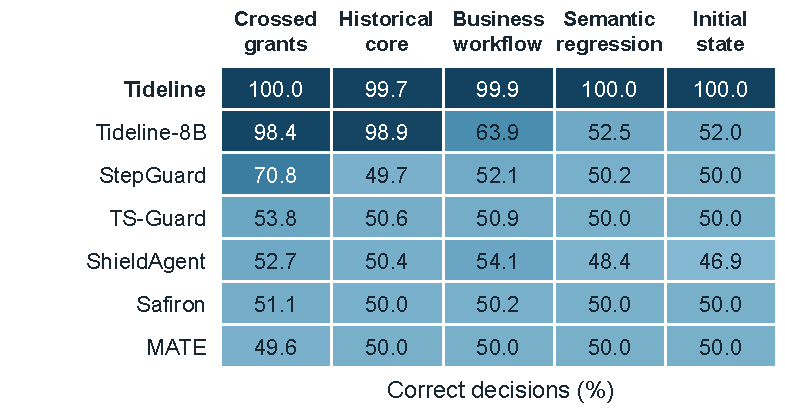
\includegraphics[width=1.0\linewidth]{figures/source_accuracy.pdf}
\caption{Accuracy (percent) by internal source on original tasks, rounded to one decimal. Each cell weights requests within its own source. Table~\ref{tab:strata} gives exact Tideline error counts.}
\Description{Seven reviewer rows and five source columns. The authorization backbone scores higher on the historical sources than on the business and state sets.}
\label{fig:source}
\end{figure}

On the original wording, Tideline-8B scored 98.4\% on the crossed-authorization batches, 63.9\% on the business workflows, and 52.5\% on the quantity-report regression requests (Figure~\ref{fig:source}). With the contextual checks, Tideline answered 2,110 of 2,112 workflow requests and all 1,920 regression requests correctly. Under paraphrase, 21 of 26 errors fell in the workflow batch (seven false blocks and 14 false allows), compared with two false blocks on the original wording. Errors on the reused training requests fell from seven to five.

\paragraph{Contextual routing counts and target-scope head.}
Across the 10,372 original contextual requests, Tideline retained Tideline-8B's default decision 5,596 times and resolved the verdict via the file-effect/permission branch 2,112 times, the snapshot precondition route 2,176 times, the literal-target path head 440 times, and a specialized count-report condition check (reading a first line, last line, or CSV field) 48 times. Across the fixed paraphrases, the corresponding counts were 5,574, 2,112, 2,176, 462, and 48. The literal-target path head applies a two-leaf decision tree fitted on 142 original historical items (124 allow, 18 deny across 23 association groups) from the fitting partition to verify whether a statically traced copy/truncation destination is authorized by the user task.

Table~\ref{tab:axes} counts requests by language and the input changed within each pair. Both wordings use the same programs, workspaces, and reference decisions.

\begin{table}[tb]
\centering\small
\caption{Internal requests in one wording edition. Rows indicate the diagnostic question and columns the language of the candidate.}
\label{tab:axes}
\begin{tabular}{@{}lrrr@{}}\toprule
Changed input & Shell & Python & Total\\\midrule
User request & 2,080 & 2,080 & 4,160\\
Script & 1,288 & 1,288 & 2,576\\
Initial workspace state & 1,818 & 1,818 & 3,636\\\midrule
Total & 5,186 & 5,186 & 10,372\\\bottomrule
\end{tabular}
\end{table}

\paragraph{Keeping related items together.}
The development partition grouped requests associated through a source project, quartet, program combination or business workflow. It assigned 4,190 requests to the fitting portion and 6,182 to the remainder. Both wordings of a request shared an assignment. Earlier heads used the original fitting portion. The literal-target head used 142 original historical items in that portion, comprising 124 allow and 18 deny examples from 23 association groups. Separately, the 2,112 business-workflow items supported file-level modeling. Fourteen workflows (1,232 items) were used for training, four (352) for development and six (528) for testing in that study. The partitions shared construction templates. Both wording editions informed subsequent diagnosis and selection.

\paragraph{Counting groups.}
For a group $G$ of two or four requests, complete correctness is $\prod_{i\in G}\mathbf{1}[\hat y_i=y_i]$. Average this indicator over groups of the same kind and wording. For item accuracy, instead sum the individual indicators and divide by the number of requests. The two averages need different denominators. For example, a four-cell group with three correct decisions contributes 75\% to its item score and zero to its complete-group score. Table~\ref{tab:removal} also gives the item-level counts of false blocks and false allows.

\section{Command Labels, Fitting and Paired Uncertainty}
\label{app:external}
\paragraph{Which rows enter scoring?}
The three sources supplied 4,407 identifiers corresponding to 4,404 distinct visible inputs. Reviewers assessed each distinct input twice. Mapping the votes back to identifiers gives 3,186 consensus allows, 443 consensus holds, 369 pairs of insufficient-evidence votes and 409 disagreements. The first two counts sum to 3,629. Three of those rows lacked an upstream binary label. Restricting scoring to the original binary-labeled population therefore leaves 3,626 consensus rows. The remaining 777 of 4,403 scored rows use the upstream binary label. Across the scored rows, 245 labels changed from allow to hold and 28 from hold to allow. The 4,404 distinct visible inputs used for review are a different population from the 4,403 scored identifiers.

\begin{table}[tb]
\centering\small
\caption{Reconciliation by external source in the main run. The last two columns count errors on scored identifiers.}
\label{tab:sources}
\begin{tabular}{@{}lrrrr@{}}\toprule
Source & Received & Scored & False blocks & False allows\\\midrule
ShellRisk-Bench & 4,194 & 4,194 & 72 & 50\\
shell-guard-bench & 201 & 197 & 8 & 8\\
agent-policy-bench & 12 & 12 & 0 & 2\\\midrule
Total & 4,407 & 4,403 & 80 & 60\\\bottomrule
\end{tabular}
\end{table}

\paragraph{Template groups.}
For template comparison, the normalizer substitutes a common marker for quoted spans, matched paths, selected filename forms and numbers, then normalizes whitespace. Commands sharing the resulting string have one group identity. The fitting partition covers 1,428 such templates. The held-out portion covers another 2,263. Near-equivalent commands that the normalization maps to different strings can appear across the partition. This definition also explains the distinction between a visible-input duplicate, which includes its working directory, and a shared template, which groups command text at a coarser resolution.

\paragraph{Fitting the score.}
The lexical estimator uses sublinear TF--IDF character features of length two to five. It requires a feature in at least two documents and retains up to 70,000 features. The logistic classifier uses balanced class weights and $C=6$. For tabular features, the fit retains columns nonzero in at least three training rows. The randomized forest uses 220 trees, feature fraction .55 and minimum leaf size two. The boosted model uses 125 stages, learning rate .05, depth two and minimum leaf size seven. Each fold fits these transformations and estimators using its own training rows.

For a feature set, the grid assigns lexical weight in $\{.05,.12,.20\}$ and randomized-tree weight in $\{.25,.45,.65\}$, with the remainder assigned to boosting. The threshold ranges from .220 through .660 in increments of .005. On out-of-fold predictions the search first minimizes the larger of the two error counts, then their sum, then the absolute distance of the threshold from .5. Across feature sets the first two criteria select the final configuration. The held-out labels do not enter this grid search.

\paragraph{Blind consensus review and calibration details.}
Figure~\ref{fig:label_review} shows pairwise agreement across the three randomized blocks of 1,468 unique visible commands (Cohen's $\kappa$ = 0.741, 0.752, and 0.811 for A/B, A/C, and B/C); most disagreements involved one reviewer selecting insufficient evidence rather than opposite binary votes (only 3, 3, and 5 direct flips across the three blocks). For the command-only fallback, the selected five-fold cross-validated score combines the lexical ($p_L$), randomized-tree ($p_T$), and boosted-tree ($p_B$) probabilities via $s = 0.20p_L + 0.65p_T + 0.15p_B$, issuing a hold when $s \ge 0.435$. Figure~\ref{fig:calibration} compares five-fold out-of-fold errors across all eight candidate feature sets on the 1,750 fitting items (69 out-of-fold errors for the selected configuration; 4 errors after refitting on all 1,750 items; 136 errors on the 2,653-item template holdout).

\begin{figure}[tb]
\centering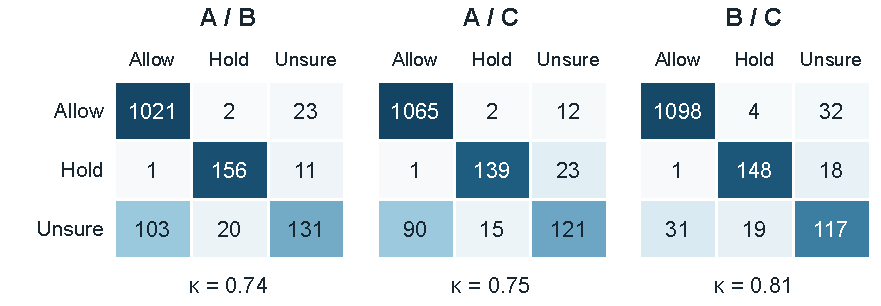
\includegraphics[width=\linewidth]{figures/label_review.pdf}
\caption{Paired blind judgments on external standalone commands before binary scoring (1,468 unique visible inputs per block).}
\Description{Three three-by-three matrices showing that most off-diagonal entries involve an unsure vote rather than opposite binary verdicts.}
\label{fig:label_review}
\end{figure}

\begin{figure}[tb]
\centering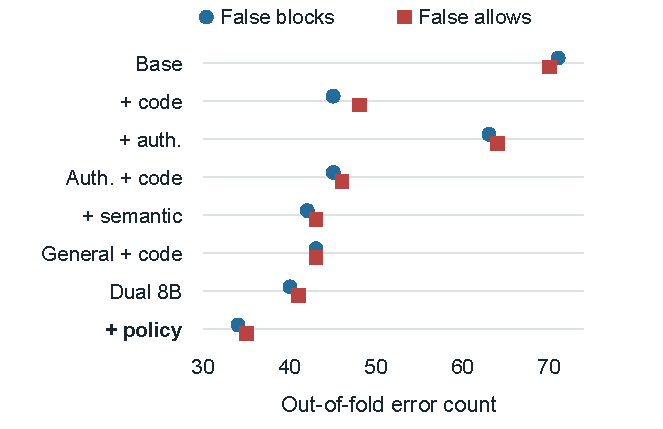
\includegraphics[width=.94\linewidth]{figures/calibration.pdf}
\caption{Five-fold out-of-fold errors across eight candidate feature sets on the 1,750 fitting commands. Dots count false blocks and squares count false allows.}
\Description{Static features yield 71 false blocks and 70 false allows; adding code encoders, language models, and operations-policy features reduces errors to 34 and 35.}
\label{fig:calibration}
\end{figure}

\paragraph{Encoder comparisons.}
For each held-out request, record whether the full and reduced configurations agree with its binary label. Count a correction when the reduced model alone is correct and a new error when the full model alone is correct. Figure~\ref{fig:turnover} reports individual decision turnover: removing the general Qwen3-8B, risk CodeBERT, and joint CodeBERT encoders corrected 22, 30, and 33 errors while introducing 38, 38, and 36 new errors, respectively. The accuracy difference in percentage points is $100$ times corrections minus new errors, divided by 2,653, with the subtraction performed before division. For uncertainty, sample 2,263 template groups with replacement and include every row in each sampled group with its multiplicity. Compute the difference on the resulting row count, which can vary across draws. Each configuration uses the same sampled groups as its comparator. We used 10,000 draws with seed 20261121. The individual intervals are the 2.5th and 97.5th percentiles. The simultaneous comparisons use Bonferroni-adjusted percentile tails of $2.5/3$ percent each.

\begin{figure}[tb]
\centering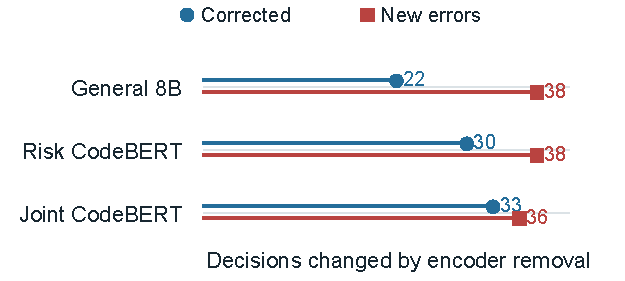
\includegraphics[width=\linewidth]{figures/turnover.pdf}
\caption{Individual decision turnover on the 2,653-item template holdout after retraining without one encoder.}
\Description{Removing the general, risk, and joint encoders corrects 22, 30, and 33 errors while introducing 38, 38, and 36 new errors.}
\label{fig:turnover}
\end{figure}

\section{Public Reviewer Adapters, API Protocol, and Resource Measurement}
\label{app:resources}
For each contextual request, the adapter supplies a user task, a shell tool with command and working directory, local code, and state containing the project documentation and supporting files. The requesting agent's subsequent messages and the evaluator's observations are unavailable at this point. StepGuard and MATE use their corresponding prompt builders and verdict parsers. The TS-Guard adapter supplies three fields for the task, action and environment. It maps a warning or a maximum-risk score to hold. The Safiron adapter serializes the candidate as a single agent action with environment information. ShieldAgent receives the available evidence and the trace prefix ending at the proposed tool call. An invalid verdict counts as an incorrect item in the accuracy denominator. Safiron produced one such verdict among the 10,372 original internal requests.

\subsection{Offline API Baseline Protocol and Parsing Reconciliation}
\label{app:api-protocol}
Both API baselines operated on the exact same frozen visible inputs as the checkpoint adapters across all 25,151 requests (10,372 original internal, 10,372 fixed paraphrase, and 4,407 external, of which 4,403 carry binary scoring labels). Codex Auto Review invoked request model ID \texttt{codex-auto-review} through the Responses API, and Sonnet~5 (low) invoked \texttt{claude-sonnet-5} through the Messages API (\texttt{thinking.type=\allowbreak adaptive}, \texttt{output\_config.effort=\allowbreak low}, \texttt{max\_tokens=\allowbreak 4096}). Both were routed through a third-party API gateway whose responses returned matching model IDs. Neither run recreated native client reviewer prompts or executed interactive agent sessions, and no response was resampled on correctness or format.

Many Sonnet~5 (low) responses included explanatory prose alongside a JSON verdict, causing whole-string strict JSON parsing to fail on 7,488 of 25,151 responses. Under the unique explicit-decision extraction rule, surrounding text is accepted only when all explicit decision values in parsed JSON objects agree on \texttt{allow} or \texttt{deny}. This rule recovers 7,410 format-only responses while keeping 78 invalid responses unrecovered: 52 with conflicting or unknown decisions, 17 with no explicit JSON decision, and 9 incomplete responses. Invalid responses are counted as incorrect rather than remapped to denials. Table~\ref{tab:api-parsing} summarizes these counts by evaluation group. Applying the identical explicit-decision rule to all 25,151 Codex Auto Review responses leaves every decision unchanged (0 invalid).

\begin{table}[tb]
\centering\small
\setlength{\tabcolsep}{4pt}
\caption{Sonnet~5 (low) invalid responses under unique explicit-decision extraction across all 25,151 requests (7,488 whole-string strict parse failures, 7,410 recovered, 78 remaining invalid: 52 conflicting/unknown, 17 missing decision, 9 incomplete). Codex Auto Review had 0 invalid responses under the same rule.}
\label{tab:api-parsing}
\begin{tabular}{@{}lrr@{}}\toprule
Evaluation group & Requests & Invalid\\\midrule
Internal, original wording & 10,372 & 40\\
Internal, fixed paraphrase & 10,372 & 29\\
ShellRisk-Bench (full / held) & 4,194 / 2,511 & 7 / 2\\
shell-guard-bench (full / held) & 197 / 135 & 2 / 2\\
agent-policy-bench (full / held) & 12 / 7 & 0 / 0\\\midrule
Total scored (+4 unscored) & 25,147 (+4) & 78\\\bottomrule
\end{tabular}
\end{table}

The resource measurement starts after model initialization and warm-up (Figure~\ref{fig:cost}). Each fresh process warms up on 32 fitting requests, synchronizes the devices and resets the peak-allocation counters. Timing covers successive batches of eight, including the final partial batch. The reported mean time per item divides the sum of synchronized batch times by the number of requests. Peak allocation sums the PyTorch device peaks within that process. It measures model-side allocation across the cards and excludes memory outside the allocator. Dividing this quantity by the number of cards would answer a different hardware question. In a reversed-order verification on a second pair of RTX~5090 cards over 192 held-out requests, full Tideline took 198.3 and 198.8~ms/item while the single-GPU variant without general Qwen3-8B took 156.9~ms/item in both runs.

\begin{figure}[tb]
\centering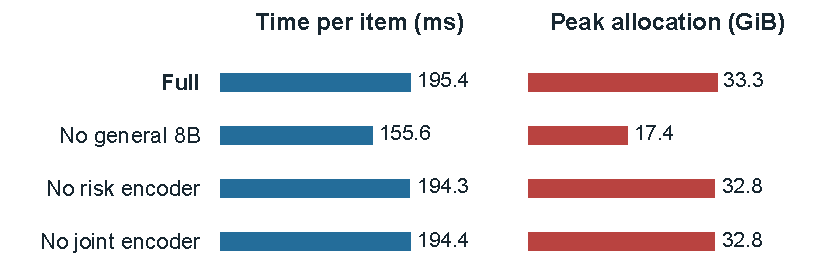
\includegraphics[width=\linewidth]{figures/resource_cost.pdf}
\caption{Amortized processing time per request and peak allocated GPU memory across command-encoder ablations on the 2,653-item template holdout.}
\Description{Removing the general 8B encoder yields the largest decrease in both latency per item and summed GPU memory.}
\label{fig:cost}
\end{figure}

\section{Continual Update Protocol, Transfer, and Policy Decoupling}\label{app:update-transfer}
Figure~\ref{fig:continual-updates} illustrates how our continual-learning pipeline constructs single-factor paired update cases verified by before-and-after workspace snapshots while keeping Tideline-8B's 8B encoder frozen~\cite{rolnickreplay,raasfig}. Each illustrative grid isolates one factor under active host policy rules. In the tool-update grid, versions v2-R and v2-A add department~A index writes to the requested report, so a report-only request permits v1 alone. In the task-grant grid, holding v2-A fixed, naming department~A authorizes the append while naming department~B withholds it. In the warehouse-stage grid, opening, sealing, and reopening a count sheet flips permission for the same inventory request.

\begin{figure*}[t]
\centering
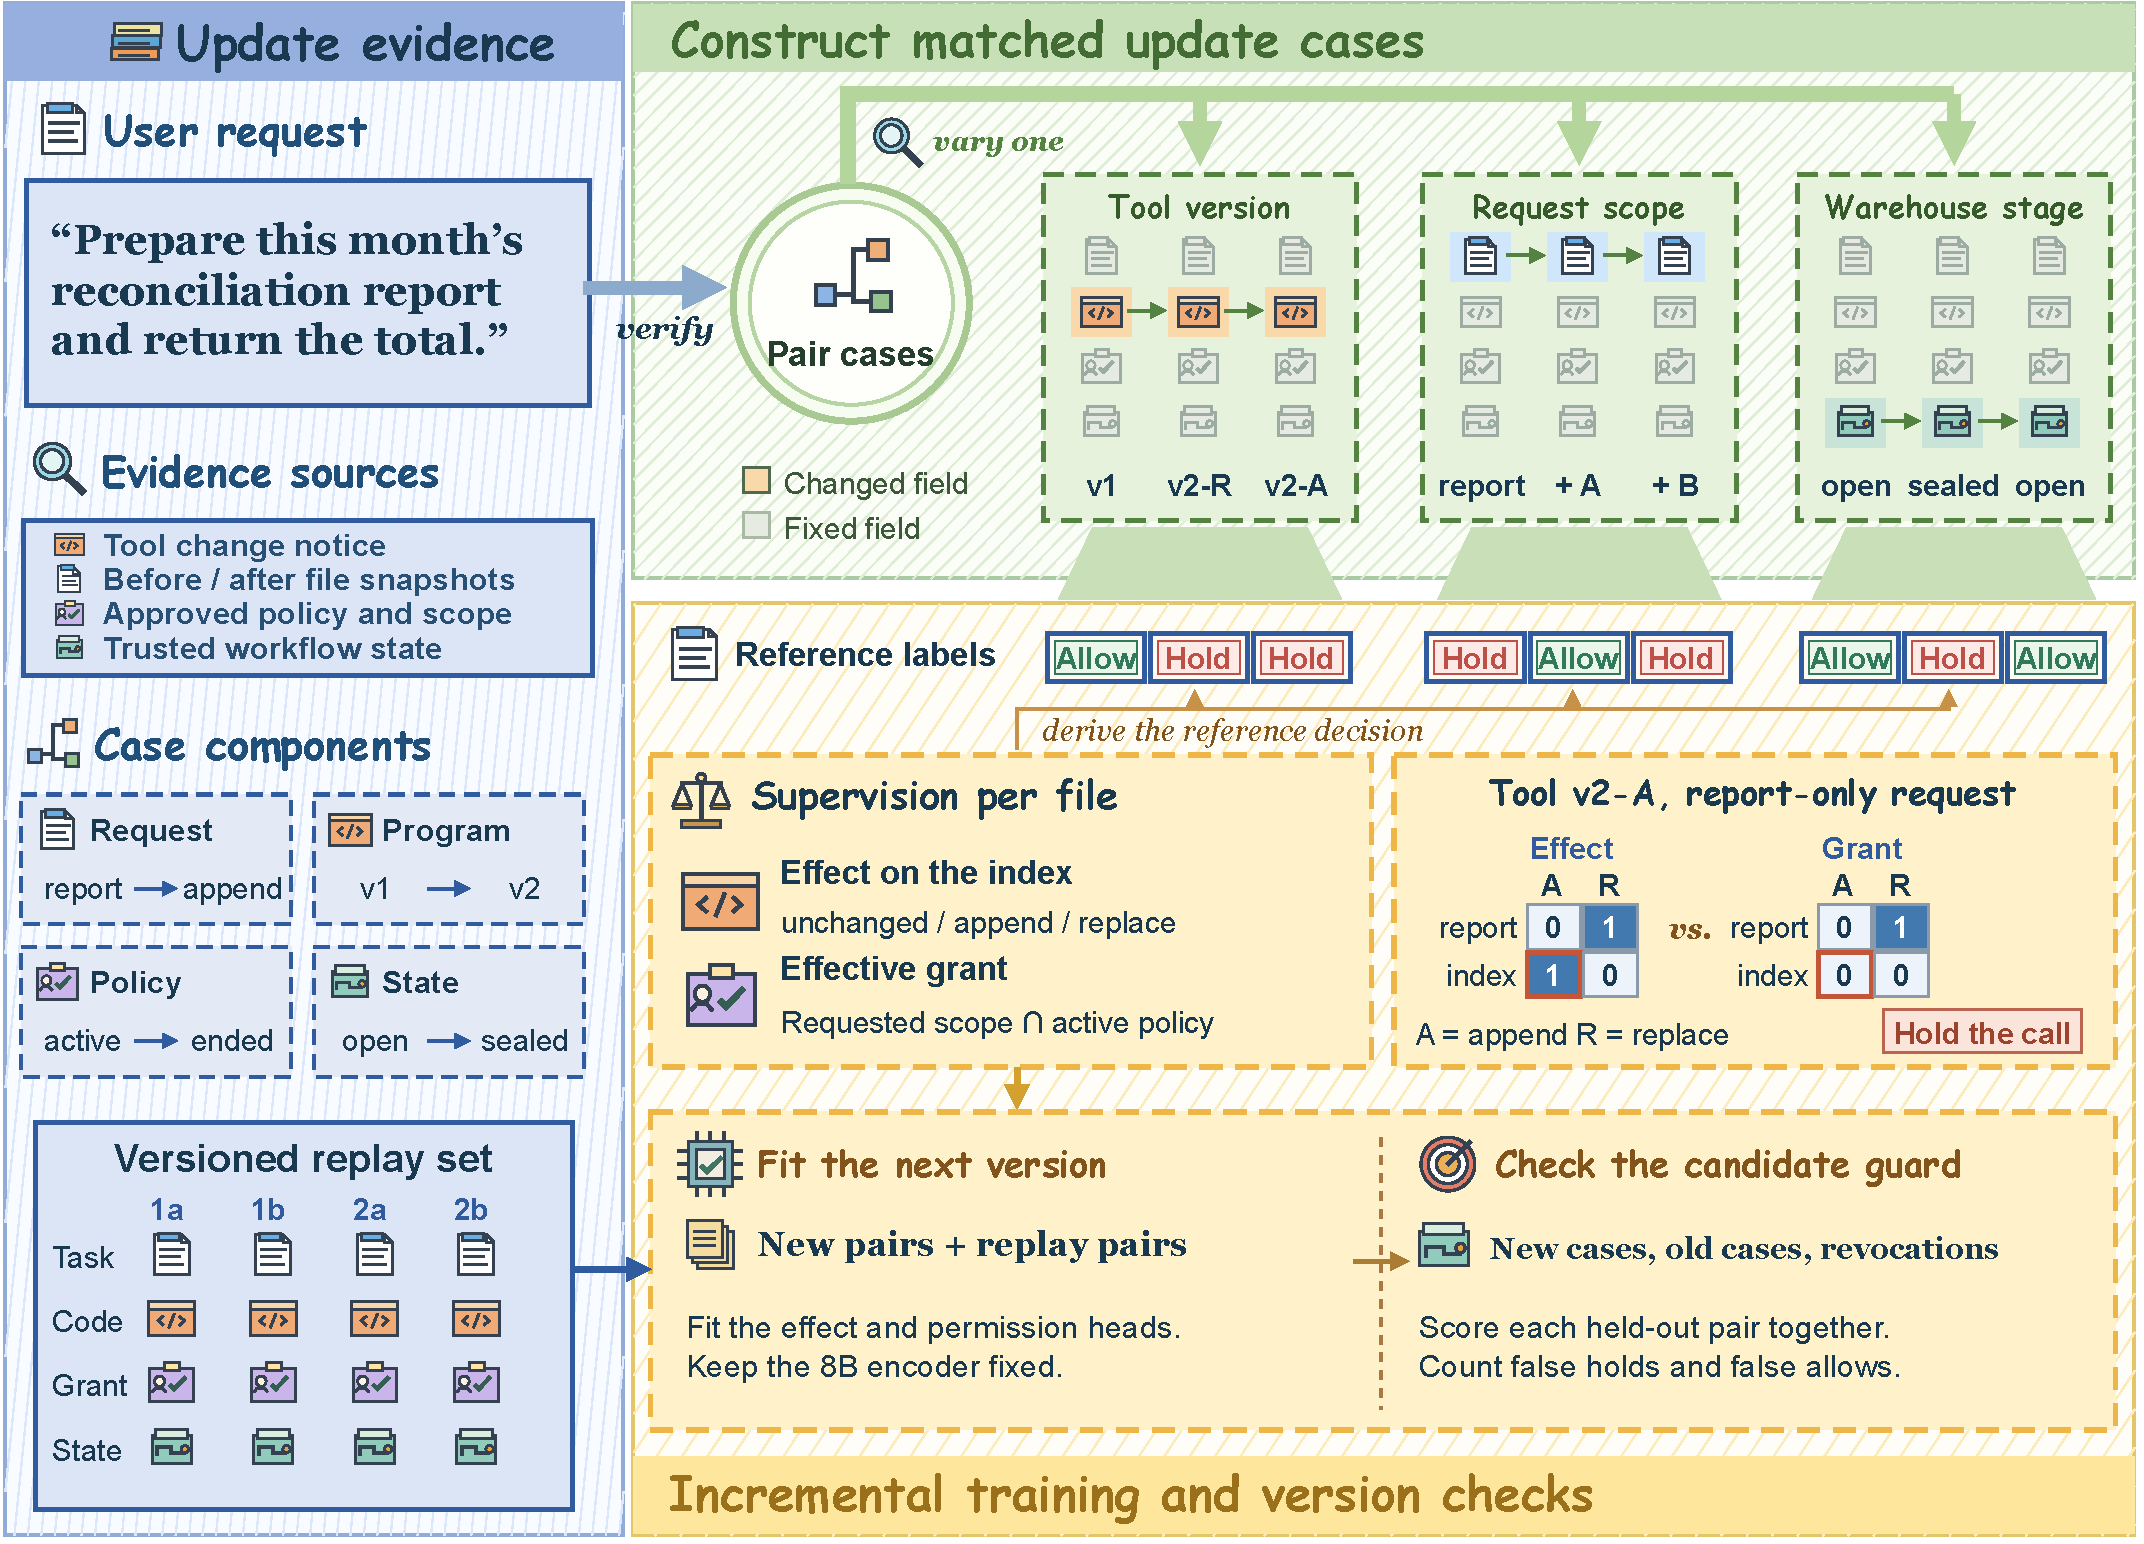
\includegraphics[width=\linewidth]{figures/continual_updates.pdf}
\caption{Versioned continual-learning protocol for Tideline. Paired cases illustrate expected decisions that isolate tool updates, task grants, and workflow states under snapshot verification and experience replay~\cite{rolnickreplay}. Panel layout adapted from Yang et al.~\cite{raasfig}, Fig.~2.}
\Description{Single-factor paired examples compare tool behavior, user requests, and workflow states with append and replace indicators. In the tool v2-A worked example, the matrices record verified file changes (report replacement and index append) against an effective grant covering report replacement only, yielding a hold target. The update loop initializes both file readouts from the prior version, keeps the 8B encoder fixed, replays policy-versioned pairs after rechecking revoked permissions, and retains the active policy on model rollback.}
\label{fig:continual-updates}
\end{figure*}

Separate from the illustrative grids, we measured a sequential update across 60 tool-version cases, 60 authorization cases, and 28 warehouse cases, evaluated on 204 held-out Shell and Python calls (96 authorized and 108 requiring a hold). Prior to updating, the frozen readouts missed 18 unauthorized calls and issued 62 false holds. With experience replay at seed~41, missed holds dropped to 0/108 and complete three-call tool-version groups rose from 7/12 to 9/12, while false holds shifted from 62 to 81, opposite-label pairs shifted from 28/120 to 24/120, and unseen request-scope and warehouse-stage groups remained at 0/12. Tracking both missed holds and false holds in that measurement established the two-sided evaluation protocol used in Section~\ref{sec:rq4}.

A rollback test held the current policy fixed after revoking a delegate's right to append to an index. The updated heads held all 12 affected calls. Restoring the original weights allowed two calls to change the index despite the revocation. An additional check held a call when a grant had been withdrawn and static analysis could not establish its complete effects. It prevented both writes and also held all 12 report-only controls, eight of which the rolled-back reviewer had allowed.

We next took cancellation actions for 20 retail orders and 13 airline reservations from the $\tau$-bench test trajectories~\cite{taubench}. The guard saw the proposed change as a replacement of the principal record, with eligibility supplied from the published policy. On copies of the upstream databases, the seed~41 replay model blocked all 33 ineligible cancellations and ran all 33 refund inquiries as well as the 33 confirmed cancellations. Frozen and current-batch heads made the same decisions. The 33/33 eligibility pairs and 0/33 consent pairs motivated a separate transfer test on new operations.

Starting from the same seed~41 replay checkpoint, we supplied 16 cancellation pairs from distinct orders in the official retail training split. Within each pair only the user's final confirmation changed. We tested on 17 retail address changes and five airline baggage changes from the official test split. The upstream tools verified that each proposed update changed the intended record in the initial database. Each object supplied two pairs that shared a confirmed request, one paired with an inquiry and the other with an explicit refusal. The experiment uses published actions, arguments, and objects together with constructed confirmation exchanges and single-action labels.

\begin{table}[!ht]
\centering\small
\caption{Fully correct pairs after fitting 16 retail cancellation pairs. Entries list counts for seeds 41, 73, and 109 in order. Each column gives its denominator. All updates start from the same parent.}
\label{tab:continual-transfer}
\begin{tabular}{@{}lccc@{}}\toprule
Update regime & Retail (/34) & Airline (/10) & Prior file (/120)\\\midrule
Common parent (seed 41) & 14 & 0 & 24\\
Current batch only & 28, 34, 24 & 0, 0, 0 & 0, 0, 0\\
Paired replay & 34, 19, 34 & 0, 8, 0 & 24, 24, 24\\\bottomrule
\end{tabular}
\end{table}

Table~\ref{tab:continual-transfer} shows that cancellation supervision improved address-change consent decisions at all three seeds, and replay retained the parent's 24 correct file pairs while current-batch updates retained zero. Across the five airline objects, replay yielded 0, 8, and 0 correct pairs out of 10. Seed~73 also missed 15 retail requests that required a hold. With seed~41 and replay, direct execution through the gate applied all 17 confirmed address changes and blocked the other 34 address requests. The same gate blocked all 15 baggage requests, including the five authorized updates.

For the OpenFGA study in Section~\ref{sec:rq4}, we enumerated all 1,603 boolean Check assertions from 54 test stores across 40 parent directories at commit \texttt{6802b4d8}~\cite{openfgastores}, normalizing to 51 distinct policy models. Running OpenFGA CLI~v0.9.0 reproduced 1,603/1,603 authored labels. Deduplicating identical policy text, effective tuples, requests, and contexts left 1,548 distinct public checks (971 allowed, 577 denied, and 62 with extra context), all 1,548/1,548 reproduced from normalized inputs. Pairing each public check with six local Shell and Python variants (report-only, log-append, log-replace) produced 9,288 derived local requests (4,250 requiring a hold and 5,038 authorized) spanning 12 source implementations, two equivalent condition phrasings, and 72 distinct encoded effect views.

Pre-update evaluations across all 9,288 derived requests clarify the architectural division between host policy evaluation and file-effect readouts. Reading host permission status alone reached 6,192/9,288 with 1,942 missed holds and 1,154 false holds (0/1,548 all-six checks), whereas static parsing that holds unresolved writes reached 4,250/9,288 with 0 missed holds and 5,038 false holds (0/1,548 all-six checks). Pre-update replay readouts scored 4,284/9,288 with 7 missed holds and 4,997 false holds (1/1,548 all-six), and disabling the condition evaluator gave 4,279/9,288. Presenting raw OpenFGA policy text and tuples directly to the file branch without host evaluation on the 1,548 append checks (max 1,043 tokens, zero truncation) triggered the condition evaluator zero times and caused the pre-update readouts to hold all 1,548 items (577/1,548 correct, versus 652/1,548 for an earlier readout checkpoint). Delegating authorization graph evaluation to OpenFGA while restricting readout learning to file effects and host-state checks avoids forcing the 8B file heads to solve external policy graphs from text.

In the four-window streaming update (34 policies split 9, 9, 8, and 8, totaling 1,064 checks and 6,384 pre-feedback items under seed~41), 8 checks per window (32 checks total) were selected by deterministic stable-ID ordering after excluding checks whose joint encoded inputs reoccurred in another window or the holdout, without using test labels. Pre-feedback accuracy across all four windows was 2,954/6,384 for frozen readouts (5 missed, 3,425 false holds, 1/1,064 all-six), 4,647/6,384 for current-batch fitting (0 missed, 1,737 false holds, 218/1,064 all-six), 4,333/6,384 for paired replay (0 missed, 2,051 false holds, 266/1,064 all-six), and 5,600/6,384 for exact-verdict memory (0 missed, 784 false holds, 823/1,064 all-six). Because exact-verdict binary memory covered all 24 observed keys in the shared-style update, we ran the reciprocal crossed-style evaluation as a follow-up diagnostic. Each fold started independently from the same pre-update checkpoint, received 32 checks (192 feedback requests) in its own style across four windows at seed~41, and held out scripts absent from that fold's new feedback (though those language constructs had appeared in earlier training of the initial checkpoint). Each source check yielded all six variants within a single test fold, and pooling the disjoint test items from both folds gave the 2,904 held-out decisions. Fold~0 trained on \texttt{printf} and \texttt{open} and tested on \texttt{echo} and \texttt{Path.open} (1,476 requests across 246 checks), lifting item accuracy from 692 (frozen and memory) to 1,045 (current) and 1,249 (replay), with complete all-six checks rising from 0 to 43 and 58 out of 246. Fold~1 reversed the styles (1,428 requests across 238 checks), raising accuracy from 638 (frozen and memory) to 1,032 (current) and 1,188 (replay), while all 238 Python report-only items received false holds when \texttt{open} was held out. The shared-style experiment scored each entire window before feedback. In each crossed-style fold, we scored the 48 selected requests in each window before updating on them. For live gating we selected the first check in stable ID order for each OpenFGA verdict present in each source file. This yielded 33 checks, for which we gated all six variants. Live execution gates evaluated those 198 requests (100 authorized, 98 prohibited): under shared-style updates, the replay gate blocked 98/98 prohibited calls and ran 93/100 authorized requests (coinciding with the offline batch on all 198 items), whereas under the crossed-style diagnostic the two corresponding fold models blocked 98/98 prohibited calls and ran 71/100 authorized requests (with two of the 198 individual replay judgments differing from the offline batch). Finally, on retention checks after the shared-style update, frozen, current-batch, and replay readouts answered 416, 412, and 404 of 528 held-out business workflow requests (58, 72, and 69 missed holds), and solved 100, 68, and 90 of 144 earlier condition-flipping pairs (8, 32, and 6 missed holds).


\end{document}
